\documentclass[]{final_report}
\usepackage{graphicx}
\usepackage{hyperref}
\usepackage{url}


%%%%%%%%%%%%%%%%%%%%%%
%%% Input project details
\def\studentname{Colin Smith}
\def\projecttitle{Using RFID to Remember}
\def\supervisorname{Lorcan Coyle, Aaron Quigley}
\def\moderatorname{Fintan Costello}


\begin{document}

\maketitle
\tableofcontents\pdfbookmark[0]{Table of Contents}{toc}\newpage

%%%%%%%%%%%%%%%%%%%%%%
%%% Your Abstract here

\begin{abstract}

\textbf{\textsl{RFID has proved to be a useful technology, becoming more common with development of
applications that benefit people in everyday useful ways. This
project demonstrates the use of this technology to aid human memory, specifically to
help people find lost items. Losing a wallet or a mobile phone is a common
occurrence for most people, and a system such as this could be beneficial. The system consists of an RFID component which identifies user interactions with objects. This data is used to help people locate lost items through interacting with a lost and
found application, which is based on human readable cues. For example, `The
user last took their wallet out of their bag at 12:00 along with their car keys'.
The cues are constructed based on interactions with such objects. Users view these cues through a web page and also receive alerts on potentially lost items through a built in system display. Results of this research indicate that RFID is a useful and effective technology in such a system. The human readable cues are found to be effective, however they can be supplemented with additional information to improve the system's overall effectiveness.}}


\end{abstract}
\newpage

%%%%%%%%%%%%%%%%%%%%%%
%%% Acknowledgments

\chapter*{Acknowledgments}

A big thank you to Lorcan Coyle, Steve Neely, and Graeme Stevenson. Thanks for all your help and ideas guys, its really appreciated. Thanks to Caitie Lustig for her work during ODCSSS and for answering all my questions. Thanks to Colm Mulryan, Olga Murdoch, Christine Trant, and Oliver van Heteren for the support during the project. Thanks to all those who participated in the cue evaluation and took the time to fill out the survey.

%%%%%%%%%%%%%%%%%%%%%%
%%% Introduction

\chapter{Introduction}
This report describes the development of the ReFInDer system, which helps users to find lost items, such as a phone or wallet. It is based on RFID technology, which is used to record user interactions with these items. RFID is a way of wirelessly identifying objects, consisting of a reader and tags. When an item is tagged, it can be uniquely identified when it comes into range of the reader. Using these records of user interactions with items, a Memory Aid can be developed. This takes the form of a web site where users can obtain information about their interactions with a lost item and aid them in remembering where they may have lost it.

ReFInDer consists of of a mobile component and a website. The mobile component consists of the RFID reader connected to a portable micro-sized computer, which has an extremely small form factor. This gathers information about users' interactions such as when they had certain items and what locations and people they have come in contact with. The static component consists of a server and lost and found website. The data gathered by the micro-computer is wirelessly transmitted to the server, stored in a database, and presented to the user through the website. The mobile component also incorporates an LCD screen, facilitating an additional user interface. In addition to the implementation steps given by the project specification an additional means of gathering information about a users' activities was explored using Bluetooth.

This report presents a detailed overview of the goals, design and outcome of the system implementation. It includes a full description of the system design and construction leading to system evaluations and conclusions. Chapter~\ref{background} discusses background research relevant to the project. The papers presented are relevant to the technologies being used and provide useful insight into related fields of research involving these technologies. The background research also gives further insight into the applicability or usefulness of RFID for the proposed system design, and explores the concepts and goals of this project. Chapter~\ref{implementation} gives a detailed description of ReFInDer's implementation. This includes the system's design with regards to the hardware being used and the system's form factor. This chapter also includes descriptions of ReFInDer's data processing techniques and overviews of the software technologies being used. Chapter~\ref{evaluations} describes how the system is evaluated and tested. This chapter describes testing which was implemented on the system's key components. Chapter~\ref{future} presents the final conclusions of this work based upon the overall evaluations and performance of the system. The applicability of this system for its intended purpose are discussed and the future research potential for this technology is explored. 

\section{Project Specification}
The following is the original specification for this project:

Title: Using RFID to Remember

Lecturer: Lorcan Coyle and Aaron Quigley

Description: Associating interactions between users and artifacts in their everyday surroundings could be a useful way of helping people remember where they left them. When people cannot find something, simple cues like `you left your keys on the dresser table', or `i saw you take your wallet with your mobile phone' are naturally helpful. This project seeks to record a person's interactions with everyday items and generate useful cues to the user when they lose something.

This project builds on an earlier ODCSSS summer school project, where an RFID reader is embedded in a glove and RFID tags are attached to kitchen implements. The reader can see when the user interacts with any item that has an attached tag and know what that item is. 

The earlier project recorded interactions with the kitchen implements and used them to detect when the user was completing a routine task (e.g., making a cup of tea). This project would have access to the outputs of that project and one of the challenges of this project would be to understand, reuse, and extend the earlier work.

Mandatory: Software must be built to recognise a human user's interactions with everyday objects. These objects would be attached with RFID tags and the user will interact with them using the rfid glove.

The software must be capable of giving useful (if simple) cues to remind the user where lost items are, e.g. `you interacted with your mobile phone at 2:01pm, 32 seconds after you interacted with your car keys and 21 seconds before you interacted with your wallet'

Discretionary: A useful way for the software to communicate with the user should be developed - this might be through a lost-and-found web page, or a display attached to the glove.

Exceptional: More complex, human readable cues should be developed, e.g., `you last had your mobile just after 2pm; you were also using your car keys and wallet at that time'.

\chapter{Background Research}
\label{background}

\section{Introduction}

This chapter presents an overview of background research relevant to the project. In this chapter previous research involving RFID technology is discussed. The literature also explores a number of relevant concepts such as ubiquitous computing and wearable technology. These papers give a positive insight into different implementations of the proposed technologies, leading to some important conclusions on the application of RFID technology in this project.

\section{An Introduction to RFID Technology}

RFID is a technique for wirelessly identifying objects, which has become increasingly recognised for its many potential mainstream applications and uses. Examples include retail security systems and inventory management. The increase in the use of RFID is due mainly to lower cost of RFID components and the large amount of potential applications of RFID technology. Recent research into the applicability of RFID include short range mobile phone communication, and anti counterfeit cryptography and authentication techniques \cite{intel, wong}. There are various types of RFID available, suited to different types applications. From the highest level RFID can be divided into two classes, active and passive~\cite{intel}. The difference between them is based on the technique in which the tags are powered. Figure~\ref{fig:readertag} shows the RFID reader used in this system and an example tag. 

\subsection{Passive Vs Active RFID}
The RFID method used in the ReFInDer system is known as passive RFID \cite{intel}. This is opposed to active RFID where the tags contain their own power source. As these tags are much larger and will eventually require maintenance such as battery replacement passive RFID is the ideal choice. In this technique tags are powered by the reader using a method known as electromagnetic induction, essentially building a charge from the readers magnetic field. Once powered the tag can transmit its unique hexadecimal ID. Passive RFID tags are much smaller and flexible, thus more suitable for placing them on common items. They are unobtrusive and could, for example, be placed inside the battery cover of a phone. This proves consistent with the projects main goals. 

\begin{figure}[h]
\centering
\fboxsep 1mm
\framebox{
	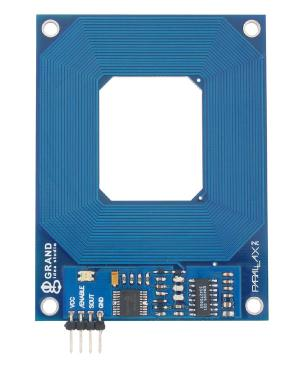
\includegraphics[width=6cm, height=8cm]{reader} 
	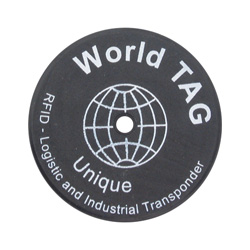
\includegraphics[width=5cm, height=5cm]{tag}
}
\caption{Left) RFID reader used in ReFInDer: measures 62.22mm x 82.5mm, Right) Example RFID tag: measures 50mm in diameter\cite{parallax}}
\label{fig:readertag}
\end{figure} 

\section{The Computer for the 21st Century}

Mark Weiser's seminal paper on ubiquitous computing proposes the concept of `embodied virtuality'~\cite{weiser}. He describes how in today's world information is everywhere in our environment, so much so that we do not even notice it. Technology is also a common element in our environment but it has yet to reach its full potential. He conceives a system in which computers cover free surface spaces in our surroundings, connected through an invisible network, and become part of our normal environment. One is surrounded by technology, but it vanishes into the background so as its presence is not noted. Such a system has countless applications. This is similar to the ideas of Dey et al. \cite{dey} in which the concept of technology integrating and blended seamlessly into our environment is explored. Weiser's proposed system identifies people through badges, for example, and adjusts the environment based on the preferences of the individual. A person enters a room and their calls and messages are automatically transferred to them through the environment. When a person enters their place of work they are identified, at which point their office logs them in and displays documents and files, or perhaps starts to make coffee, before they have even arrived.  An important point Weiser raises is that such complex systems do not require the use of complex artificial intelligence techniques. All these systems can simply be derived from knowing basic information about a persons' activities~\cite{weiser}. This project proposes a similar concept. From knowing simple information about a user's interactions with objects, a more complex and useful application can be derived. 

\section{Chatchayanuson's Kitchen Tracker}

Chatchayanuson et al.'s Kitchen Tracker system proposes to aid people with grocery shopping~\cite{ece}. The system consists of stationary RFID readers in a kitchen and tags placed on key grocery items within it. As items are removed from the kitchen, i.e., used or thrown away, the RFID readers are used to identify these items. This data is used to assist in grocery shopping indicating key items that are needed in the kitchen through real time synchronisation with a phone or PDA. These implementations are based on smart home concepts \cite{ece}. The system is an integrated and useful system contained within a home environment, assisting in every day tasks without being obtrusive to a person's life. An important point raised by this implementation is that such technologies should be unobtrusive and blend naturally into our environment. 

\section {Ubiquitous Memories}

Kawamura et al.'s Ubiquitous Memories is an innovative system designed to augment human memory through interaction with objects, and explores the area of wearable computing \cite{ubi}. From a hardware perspective the system consists of a head mounted display over the left eye for displaying video to the user. This eyepiece also incorporates a camera to record users' activities and experiences. There is an RFID reader on one wrist to read tagged objects. These are both connected to a remote control for the system which connects to a hip-mounted wearable computer. This is shown in figure~\ref{fig:borg}. This computer connects wirelessly to a LAN.
The system records the user�s experiences and activities and passes them to a server to be stored in a video database. Objects related to specific events are RFID tagged. When a tag is read the system replays a video related to that object, mimicking the behavior of human memory. When people touch objects they often recall associated memories.

\begin{figure}[h]
\centering
\fboxsep 2mm
\framebox{
	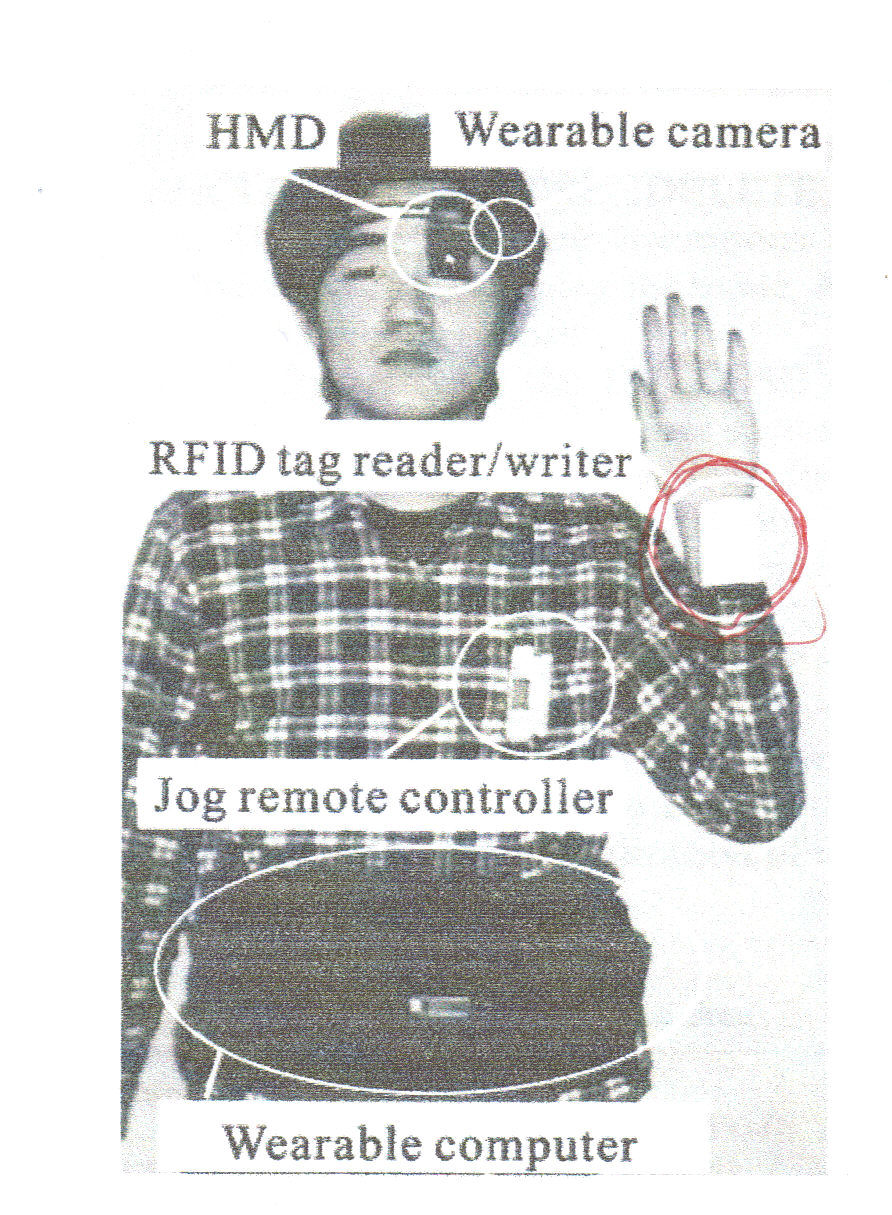
\includegraphics[width=6cm, height=8cm]{borg}
}
\caption{`Ubiquitous Memories' system\cite{ubi}}
\label{fig:borg}
\end{figure} 

The system was tested using memory and recall techniques using different memory aids. This determines the effectiveness of the system in aiding human memory and also offers insight into alternative ways of achieving this. The system is compared to other methods, in this case memory recall techniques that do not involve technology. Instead of simply rating the system performance based solely on testing it for what it is designed for, it is compared to these other methods which are designed to achieve the same goal. This knowledge could be potentially used to refine or augment the system in the future. It is this authors opinion that, like the kitchen tracker system and Weiser's concepts \cite{ece, weiser}, it is important to point out that such a system needs to be unobtrusive and feel natural in our environment. This is particularly relevant for wearable computing in which the user is often in direct physical contact or in possession of the technology while they undertake everyday tasks.  

\section {Schmidt and Gellersen's RFID glove}

Like the Ubiquitous Memories system, Schmidt and Gellersen's RFID glove explores the area of wearable computing \cite{ubi, schmidt} . In this area there is often difficulty in providing computer input if systems carry high cognitive loads or
performance problems in their deployment. They explore human computer interaction using an RFID based system in an attempt to overcome the inherent shortcomings of wearable computing. The main concept is based on implicit human
computer interaction. Implicit interaction is described as actions which are not primarily
intended to be used as computer input but can still be used as such in some useful way. This is very relevant in this proposed project and similar to Weiser�s concepts~\cite{weiser}, where computer inputs are used to create a useful application. Their
implementation consists of a glove with an integrated RFID reader. Figure \ref{fig:scmidt} shows the system components. The reader is connected
through a serial connection to a wearable computer. Each RFID tag ID is mapped to specific URL, which contains a counter. Each time an object is identified its corresponding counter is increased. Their test system did not have a specific task it was simply used to explore the use of RFID in wearable computing and if it has potential future applications. 

They conclude that such an implementation effectively overcomes the traditional problems associated with user input in wearable
computing, and propose that such a system would form a sound base for implementing
practical applications of the technology~\cite{schmidt}. Their work indicates how RFID can overcome high cognitive loads which are typical of wearable technology, where the technology does not require a user's attention or interaction in order to gather useful computer input and data.  

\begin{figure}[h]
\centering
\fboxsep 1mm
\framebox{
	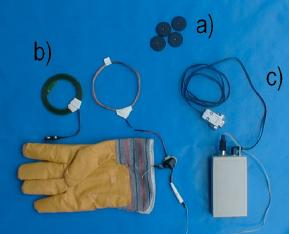
\includegraphics[width=7cm, height=6cm]{schmidt}
}
\caption{RFID glove components (from Schmidt and Gellerson \cite{schmidt}): a) RFID Tags, b) Reader Coils,
c) Wearable Tag Reader}
\label{fig:scmidt}
\end{figure} 

\section {Intel's iGlove}

In building useful applications with RFID technology a technique is required in order to allow
the computer to correctly interpret its inputs. Intel Seattle's iGlove research project explored the concept of recognising and interpreting an individuals activities from large sets of possibly related RFID readings \cite{intel2}. Like Schmidt and Gellersen, their system prototype was an RFID enabled glove with the antenna located in the palm. This is connected to a reader with radio capabilities for communicating with a computer. The glove components are all housed
in a plastic box on the outer side of the glove, which overall makes the system compact and
unobtrusive, which can be seen in figure \ref{fig:iglove}.

One difficulty their system faced was interpreting `variety', for example the same task could be completed in different ways or in a different order of steps. This would give various combinations of data inputs leading to the difficulty of interpreting them correctly. The proposed solution was to represent tasks in a sequence, or probable sequence, of the objects used, which resulted in a high level of system accuracy and performance. This is shown by their system's ability to correctly identify various tasks being undertaken by the user~\cite{intel2}. This project's proposed system also gathers large amounts of data which and similarly to this project may present inherent difficulties in interpreting it correctly, which will need consideration in the system's data processing techniques. 

\begin{figure}[h]
\centering
\fboxsep 1mm
\framebox{
	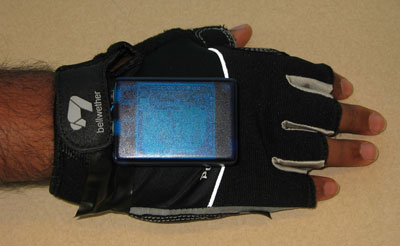
\includegraphics[width=7cm, height=5cm]{iglove} 
	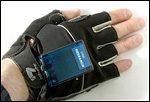
\includegraphics[width=7cm, height=5cm]{iglove2}
}
\caption{Intel's `iGlove`\cite{intel}}
\label{fig:iglove}
\end{figure} 

\section {Lustig's RFID glove}
\label{luscoyle}
Lustig and Coyle developed a similar RFID glove system following Intel's work on the iGlove~\cite{intel2}, designed to identify
specific tasks carried out by a user \cite{cait, cait2}. A glove design was implemented with an RFID reader built into the palm, as shown in figure \ref{fig:lustig}. This was connected to a micro-computer with wireless capabilities. The micro-computer can connect wirelessly to a server which in turn can update a database of tag reads and pass this information to a web page. The system is designed to recognise individual tasks by associating each one with a number of relevant tags. 

This work extends this research building upon the work already achieved while focusing on a related but different goal.  Although this project utilised some similar technologies, such as an RFID reader and micro-computer, the ReFInDer is a very different implementation and different application, specifically a lost and found application. It also explored a technique of gathering more data inputs via Bluetooth technology, and more advanced user interaction, achieved through an LCD display. Having said this it has proven useful to take into account the results and findings of their work. It was found that a glove implementation was considerably restrictive to the user, which does not conform to the principles of ubiquitous and wearable computing, which are some of the main goals of this project. This was considered a strong motivation for a new proposed form factor. 

\begin{figure}[h]
\centering
\fboxsep 2mm
\framebox{
	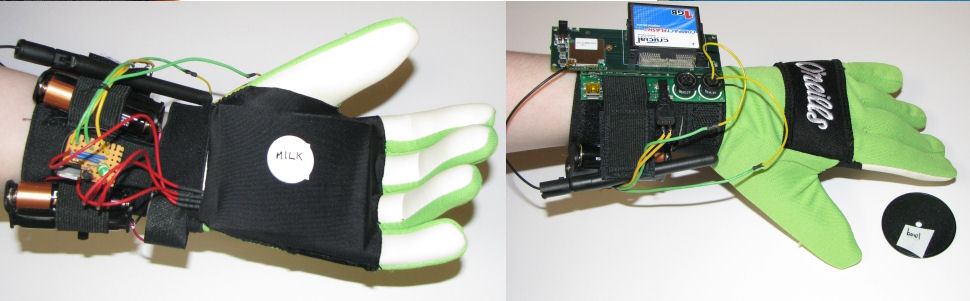
\includegraphics[width=14cm, height=5cm]{lustig}
}
\caption{Lustig and Coyle's RFID glove \cite{cait}}
\label{fig:lustig}
\end{figure} 

\section{Activity Recognition}

Logan et al. explored the abilities of different sensing equipment \cite{beth}. This research involved the use of intel's previous research on the iGlove and their later work on the iBracelet \cite{intel2, intel3}. The test system was based on a house equipped with over 900 sensor inputs, such as RFID tags, current and water flow sensors, and infrared motion detectors. The concept is also similar Lustig and Coyle's RFID glove, in that it uses sensor input to recognise human interactions and activities in a home environment \cite{cait}. In this evaluation the effectiveness of the sensor types is discussed. In the case of RFID, the user was equipped with an RFID bracelet for reading tags in the environment, sending tag reads wirelessly to a database. The results of the experiment showed that RFID performed quite poorly. It was found that this was due to the reader detecting very few of the objects being touched. There were various reasons for this, such as opposite hands being used to interact with objects, and temporary removal of the bracelet for hygiene reasons. This raises a conflicting point to the other implementations, that RFID may not necessarily be useful in some instances. For example if a person is washing dishes they cannot have electronic equipment attached to their hands~\cite{beth}.    

\section{Recognising Assembly Tasks}

Ward et al. explored the concept of activity recognition and ubiquitous computing \cite{jamie}. Mobile workers, such as maintenance personnel, often face difficulties in accessing useful information relevant to their task. For example a person may need to access a PDA to bring up schematics which requires complete physical and mental attention. The proposed concept involves identifying users' activities and automatically displaying task relevant data through a head mounted display. This involves both sound and accelerometer sensors, for gesture identification, to gather data and use different algorithmic methods to identify individual tasks. The arm mounted sensors are shown in figure \ref{fig:assembly}. One problem with this, similar to that of Logan et al., involves non relevant activities \cite{beth}. For example, while a user undertakes a task they may momentarily break from this, perhaps to take something from their pocket. Their system was tested on a `mock' scenario where a user constructs a simple item from wood. Although their results were promising they conclude that their approach would be more applicable in a home environment, especially with regards to sound identification. They propose to explore other sensor and algorithmic methods, one of which being RFID, to improve the performance of the system~\cite{jamie}.

\begin{figure}[h]
\centering
\fboxsep 2mm
\framebox{
	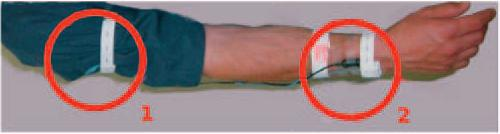
\includegraphics[width=11cm, height=4cm]{worker}
}
\caption{Arm mounted microphones and accelerometers\cite{jamie}}
\label{fig:assembly}
\end{figure}      

\section{Conclusions}
Much of this previous work in RFID applications offers some important guidance and insight for this project.
One important point raised by many of the discussed research papers is that such systems need to be
unobtrusive, feel natural to a user, and blend naturally into our environment. Ubiquitous
Memories and Chatchayanuson et al.'s kitchen tracker are good examples of this, as well as the important concept of ubiquitous computing \cite{ece, ubi}. Weiser raises another important point which is relevant to this project's system. From simply knowing some basic information, such as where you where at certain time, a more complicated and useful application can be derived, in this case a memory aid \cite{weiser}.

There are often many problems facing the concept of �wearable computing� systems, as discussed by Schmidt and
Gellerson, such as problems with performance. While this is true, it is suggested that RFID offers
a sound base for implementing practical applications of these technologies and overcoming
such associated problems \cite{schmidt}. In conflict to this, Logan et al. suggested that RFID may not be useful in some instances, however their evaluation involved recognition of many, very complex user activities, over a long period of time \cite{beth}. In the instances of low performance involving RFID it seems, in this author's opinion, that the reasons for this could have been taken into account or avoided through revising and augmenting activity recognition and sensor techniques of the system. The application in this case is also quite different to that of ReFInDer. Identifying a large number of complex tasks as a user undertakes their everyday home activities involves a high number of random factors, such as spontaneously switching between tasks. In the proposed system items are static in a certain sense, where an item is placed in a pocket within very close proximity to the reader. The possibility of not reading an item in this form factor is low in most cases, as discussed in section~\ref{evaluationsform}. It can be concluded that with this system's form factor and design, RFID technology proves very effective. 

Lustig and Coyle found their RFID system to be very restrictive \cite{cait}. This project will explore an alternative form factor in order to overcome these disadvantages. This project will use some of the proven hardware and technologies as Lustig and Coyle's earlier work, such as the micro-computer and RFID reader, but with a different implementation and application. Their system followed the work of Intel in using RFID to identify a user's activities, whereas this project proposes to gather data on a user's interactions with objects. It also takes into account more useful information, such as location and interactions with other people. Interaction between users and the system is augmented using a built in LCD screen to display relevant information.  

\chapter{System Design and Implementation}
\label{implementation}

\section{Introduction}
Chapter \ref{background} gave an overview of the applicability and suitability of RFID technology to the areas of wearable and ubiquitous computing. It also highlighted its ability to overcome the shortcomings inherent to these fields, leading to the conclusion that RFID is a suitable technology for building the ReFInDer system. This chapter describes how RFID technology is used and presents a detailed overview of the ReFInDer system's design. This includes the system's form factor and the types of hardware used. The system's data processing techniques are discussed with descriptions of how data is gathered, stored, and used in the application.   

\section{Problem Analysis}
There are two main components required in the ReFInDer system. A mobile component which is carried by the user and a web based lost and found application. The mobile component is necessary to gather information about a user's interactions with items. It requires the ability to process and wirelessly transmit this recorded data. The form factor of this component must be one which is portable and capable of performing its task with minimum user interaction. The web based component requires a means of receiving and storing recorded data. An application is needed to retrieve this information and make it accessible to the user. This application takes the form of the lost and found website and provides a user interface to the system.  

\section{System Form Factor}
The initial concept and form factor of the mobile component was an RFID enabled glove, inspired by the work of Lustig and Coyle~\cite{cait}. The major downfall of their system was the inherent restrictiveness of the glove�s design (as discussed in Section \ref{luscoyle}). Also their system was based upon a very different application, recognising user activities, where a glove design is more suitable for this task. It is also the opinion of this author that an RFID enabled glove design is very obtrusive to a user's everyday activities, and is not consistent with the ideals of technology blending naturally into our environment. 

\begin{figure}[h]
\centering
\fboxsep 1mm
\framebox{
	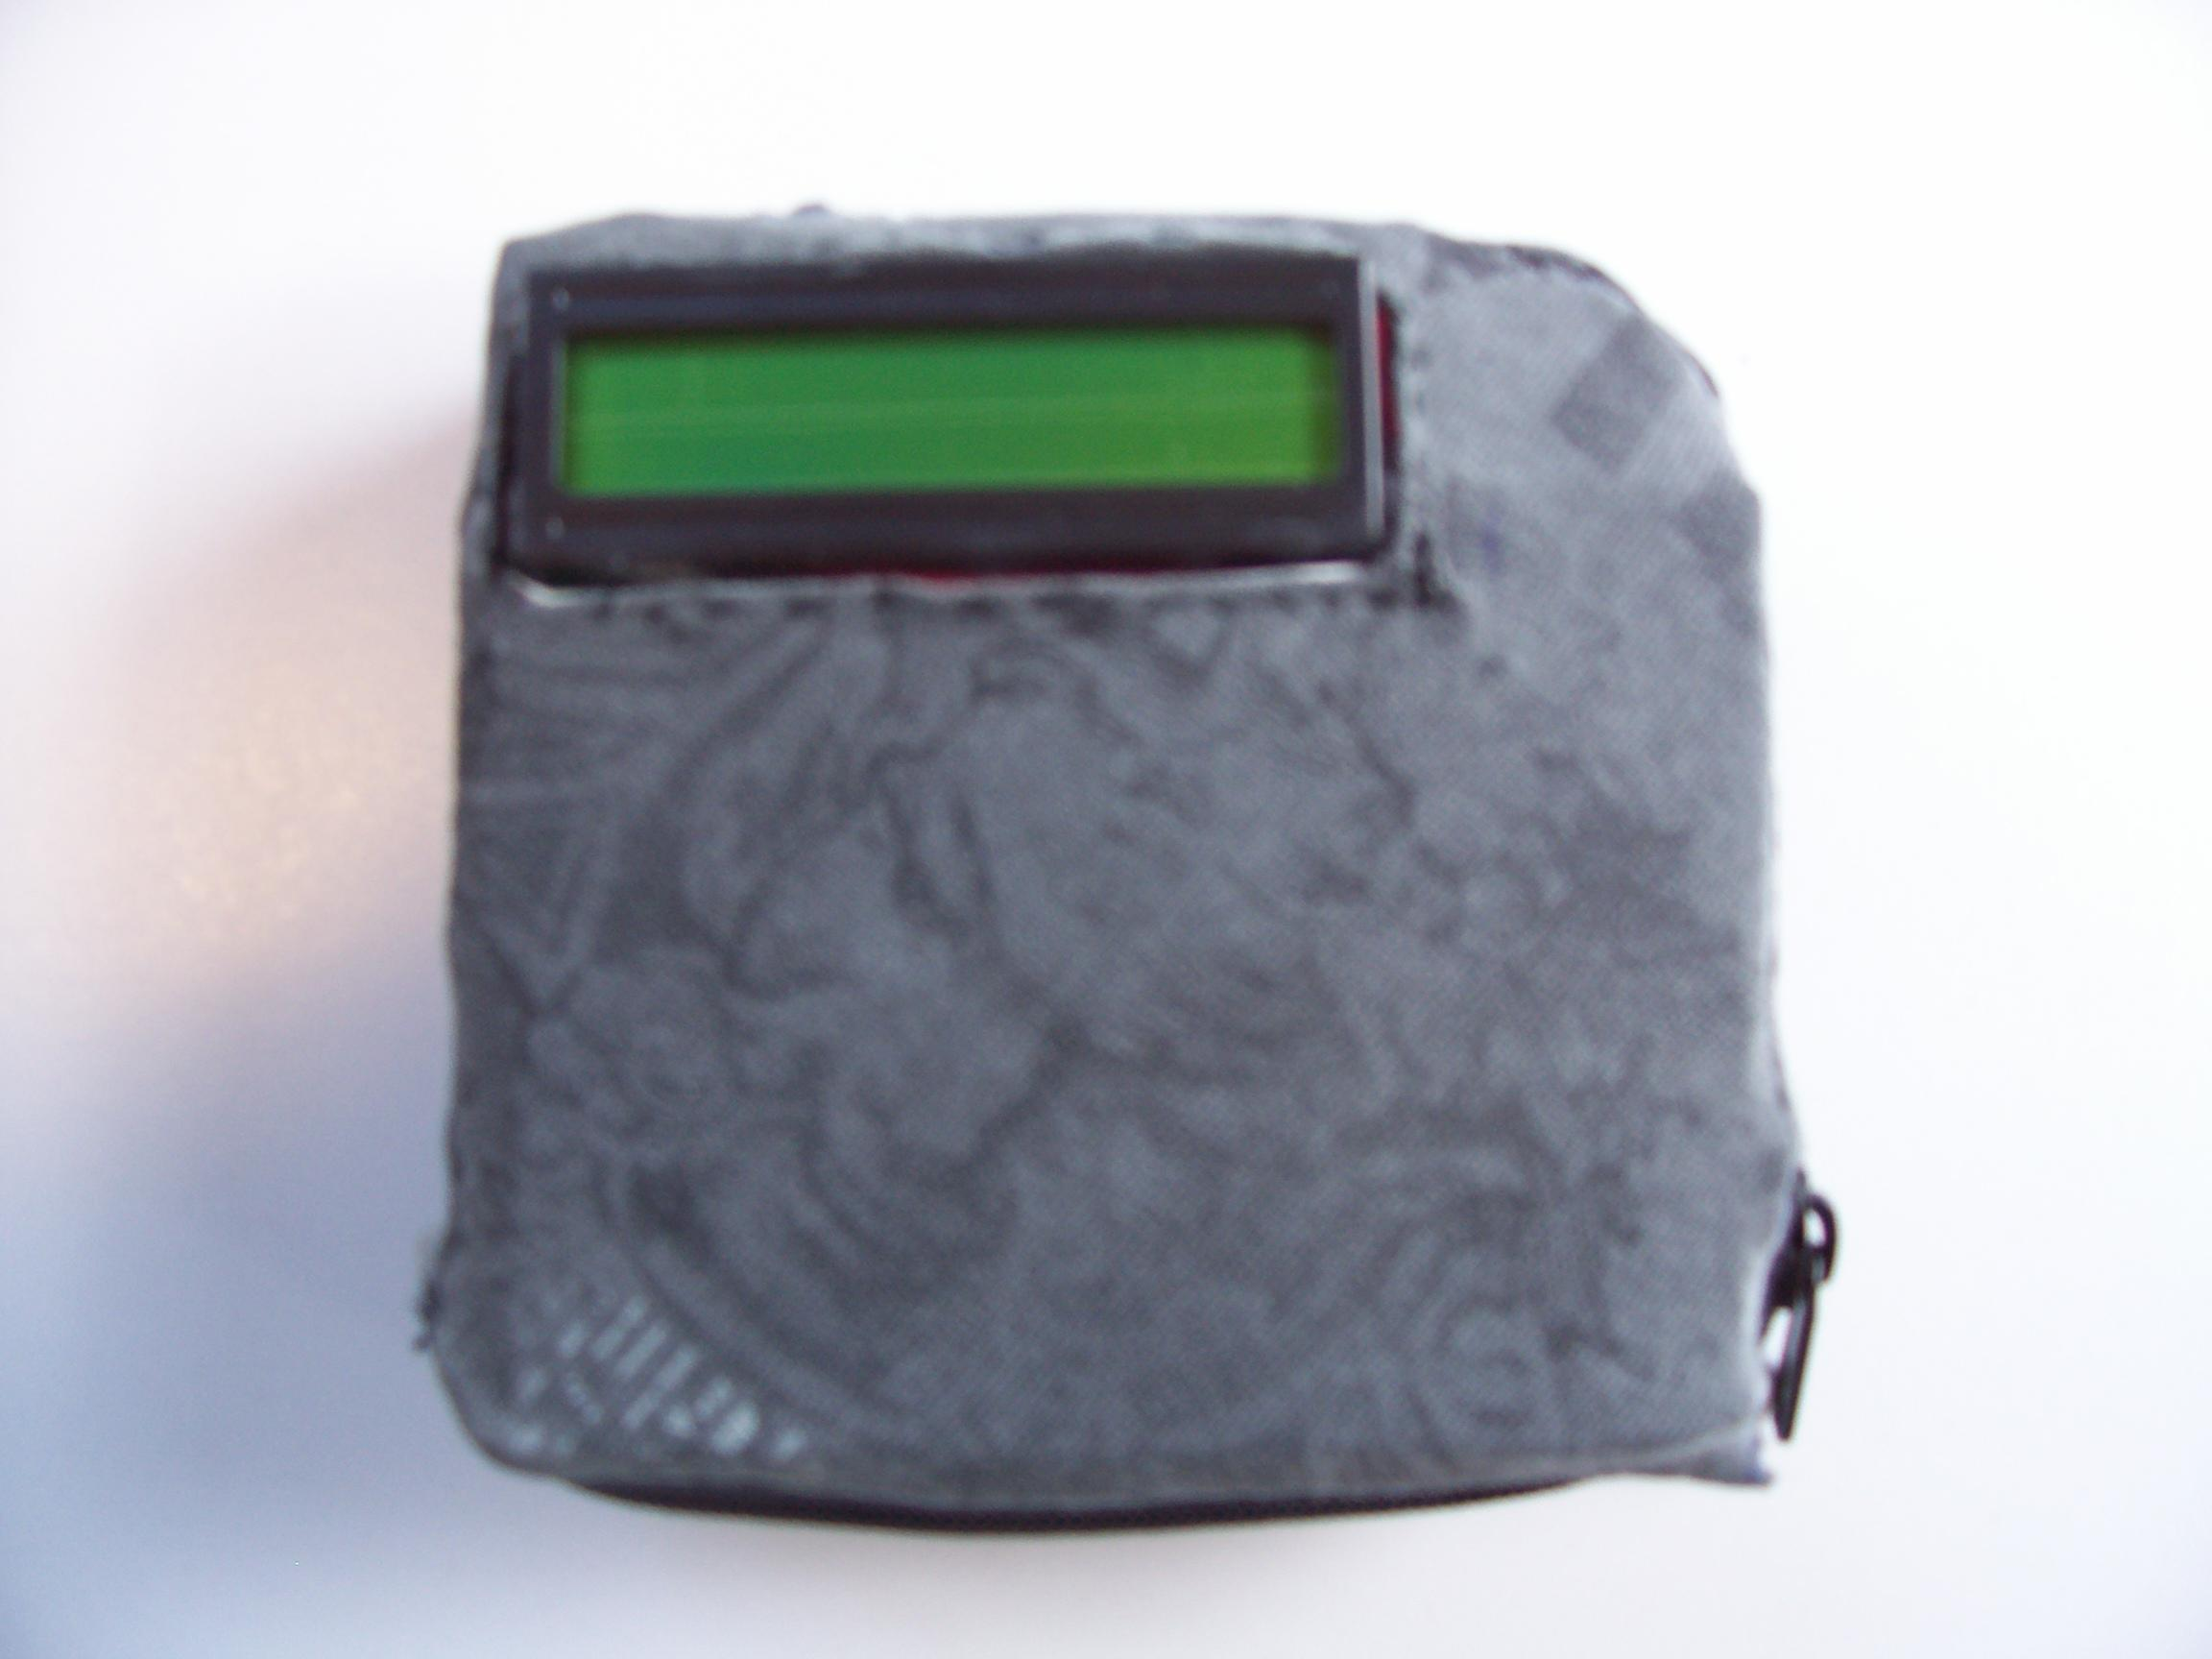
\includegraphics[width=7cm, height=6cm]{pouchfront} 
	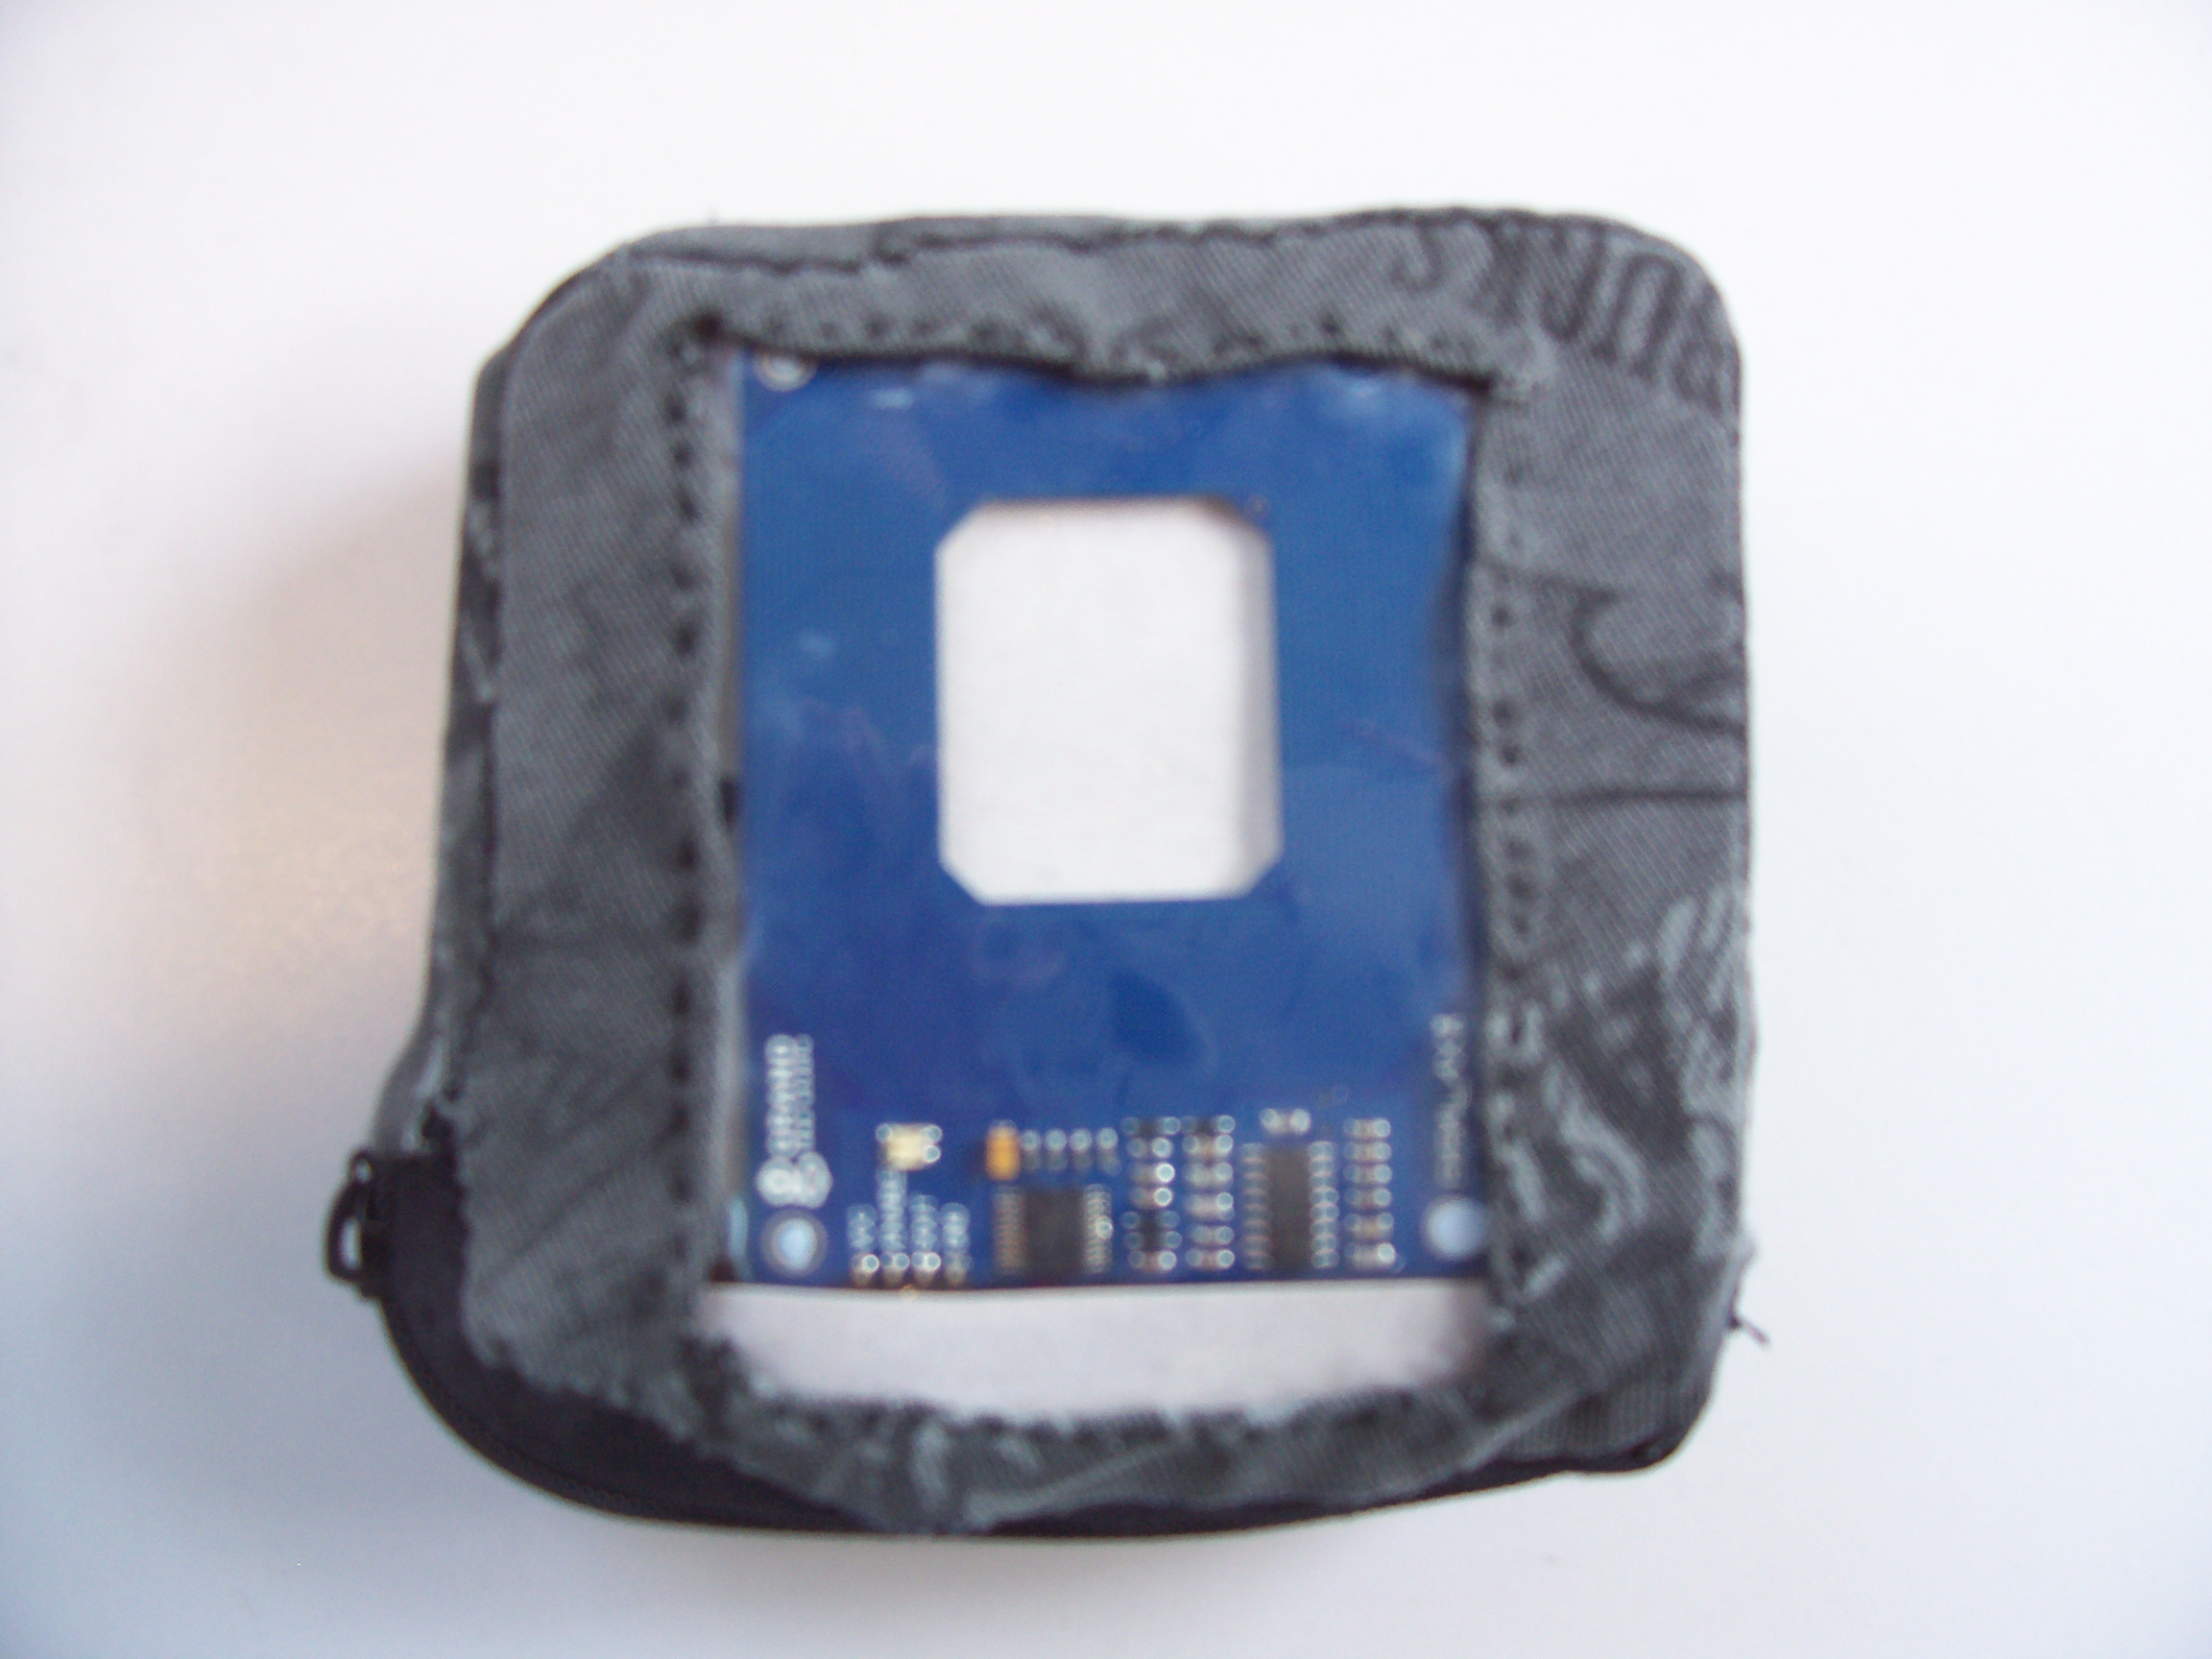
\includegraphics[width=7cm, height=6cm]{pouchback}
}
\caption{System Form Factor: Left image shows the front of the pouch with an integrated LCD display. Right image shows the back of the pouch with RFID reader.}
\label{fig:pouch}
\end{figure}

Another consideration in the design of the system's form factor arised from the initial prototype evaluation. The form factor was influenced by the inherent limitations of the RFID reader's range. This is discussed further in section~\ref{evaluationsprototype}. For these reasons a different system form factor was developed for ReFInDer. This takes the form of a pouch which is placed inside a pocket with tagged items. A box was designed using a 3D printer to house the mini computer. This box along with the RFID reader and batteries are held within the pouch. The prototype ReFInDer pouch measures 10.5cm x 11cm, and is 2.5cm thick. Its weight is 0.35kg. It is made of cloth and contains a zip at the bottom which facilitates the removal of the internal components for battery replacement. A switch is also found inside the zip for powering on and off the system. The front side of the pouch features the LCD display and the back side of the pouch has a clear plastic covering to show the RFID reader. This pouch is carried easily within a pocket or a bag. Due to the limited capacity of pockets and bags the reader will be constantly in close proximity to tagged items. The goal of this is to overcome the limitations of the reader's range. To evaluate and test this design, the pouch was placed in a bag and jacket pocket with tagged objects. The purpose of this evaluation was to determine if tagged objects could be successfully identified using this system form factor. These evaluations are discussed further in section~\ref{evaluationsform}    

\section{Hardware Design}
There are a number of key hardware components required for the ReFInDer system. The mobile component of ReFInDer consists of an RFID reader connected to a Gumstix computer~\footnote{Gumstix information can be found here: \url{www.gumstix.com}}. The Gumstix is a mini computer running a Linux operating system. The Gumstix is expanded with wireless capabilities, two serial connections, and has an integrated Bluetooth module. Expanding the Gumstix involves using expansion boards which simply click onto the Gumstix. The first board is known as a Wifistix which gives the Gumstix wireless capabilities and the second board contains two serial port connections. Figure \ref{fig:gumfun} shows these components. The Gumstix facilitates the necessary data processing and wireless transmission of recorded data required by the mobile component. It is responsible for gathering informatiion about a user's interactions with objects and transmitting this data wirelessly to the Lost and Found application. Information about a user's interactions is gathered using the RFID reader, which detects when the user is in possession of specific tagged objects (step 1 in figure~\ref{fig:architecture}). To connect the reader to the Gumstix a small circuit is constructed which regulates a 5V power supply for the reader and relays tag reads to the Gumstix through one of it's serial ports. Figure~\ref{fig:schematic1} shows the schematic for this circuit. Figure~\ref{fig:circuit} shows the circuit and the RFID reader connected to the Gumstix.

\begin{figure}[h]
\centering
\fboxsep 1mm
\framebox{
	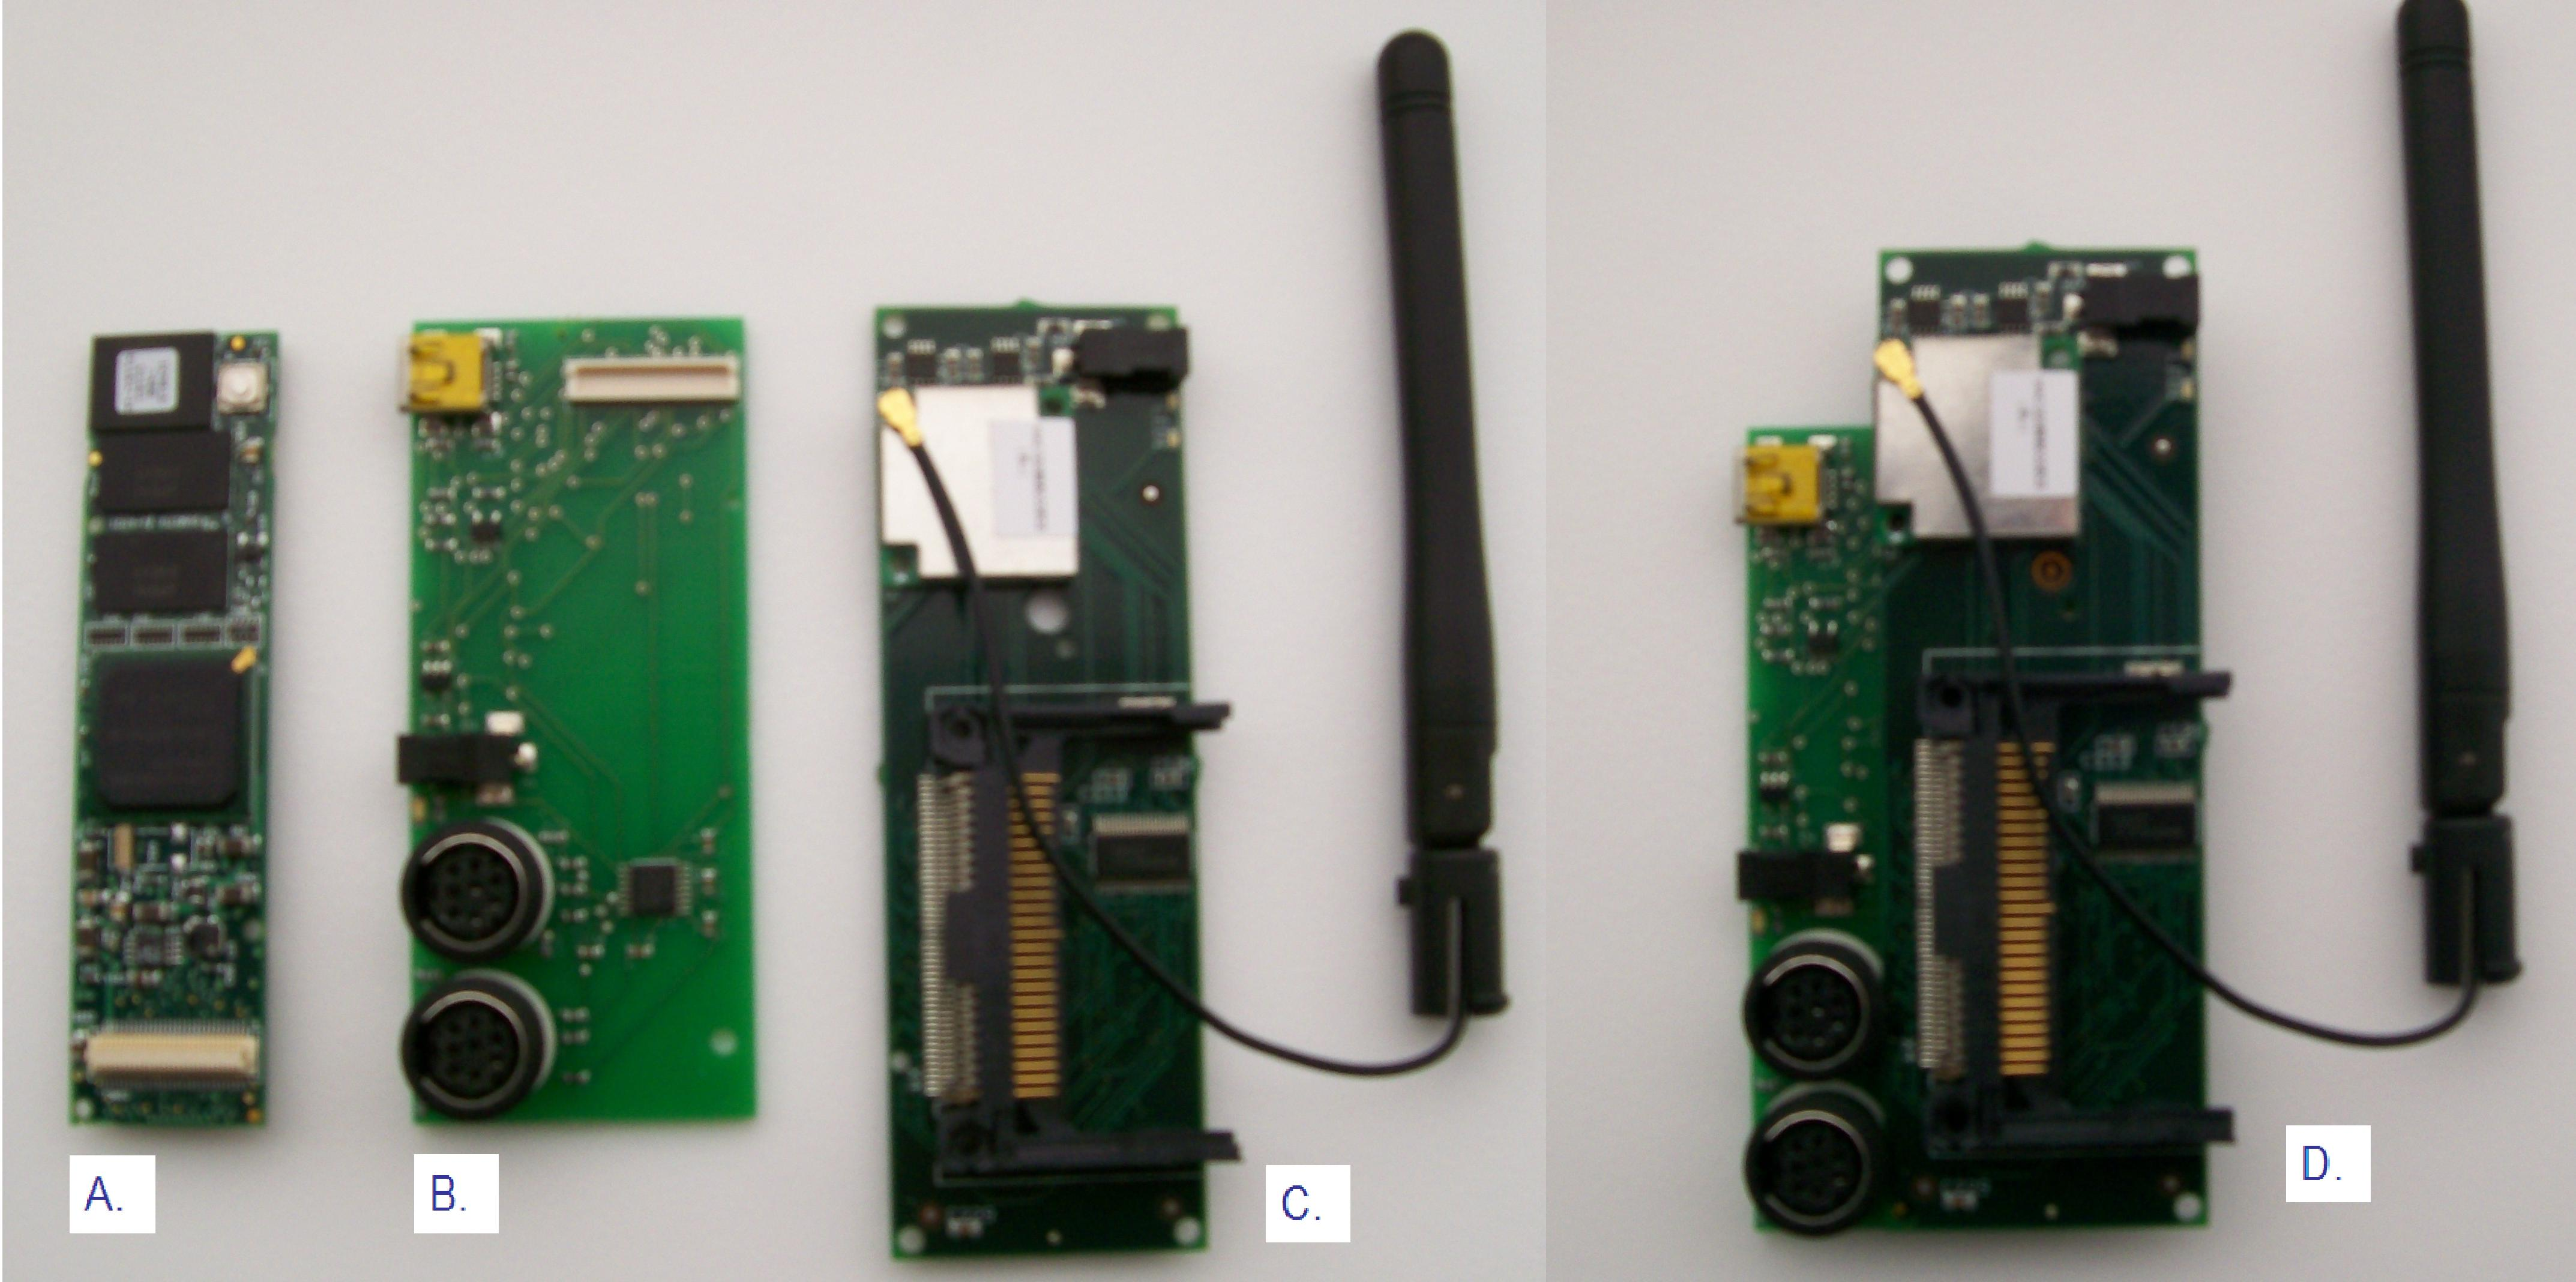
\includegraphics[width=15cm, height=8cm]{gumfun}
}
\caption{A) Gumstix, B) Serial port expansion board, C) Wifistix, D) Gumstix connected to Wifistix and Serial expansion board}
\label{fig:gumfun}
\end{figure} 

\begin{figure}[!]
\centering
\fboxsep 1mm
\framebox{
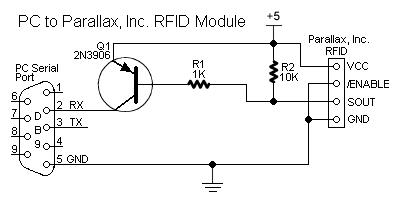
\includegraphics[width=7.5cm, height=5.5cm]{schematic1}
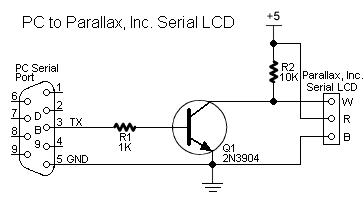
\includegraphics[width=7.5cm, height=5.5cm]{schematic2}
}
\caption{\label{fig:schematic1}{Left) Serial to RFID reader circuit schematic, Right) Serial to LCD circuit schematic\footnotemark}}
\end{figure}
\footnotetext{More information Serial to RFID schematic can be found here: \url{http://forums.parallax.com/forums/default.aspx?f=21&m=180521}}

\begin{figure}[h]
\centering
\fboxsep 1mm
\framebox{
	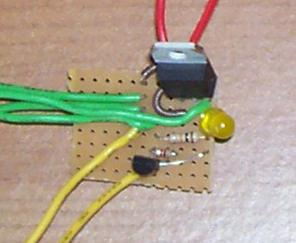
\includegraphics[width=7cm, height=7cm]{circuitShot} 
	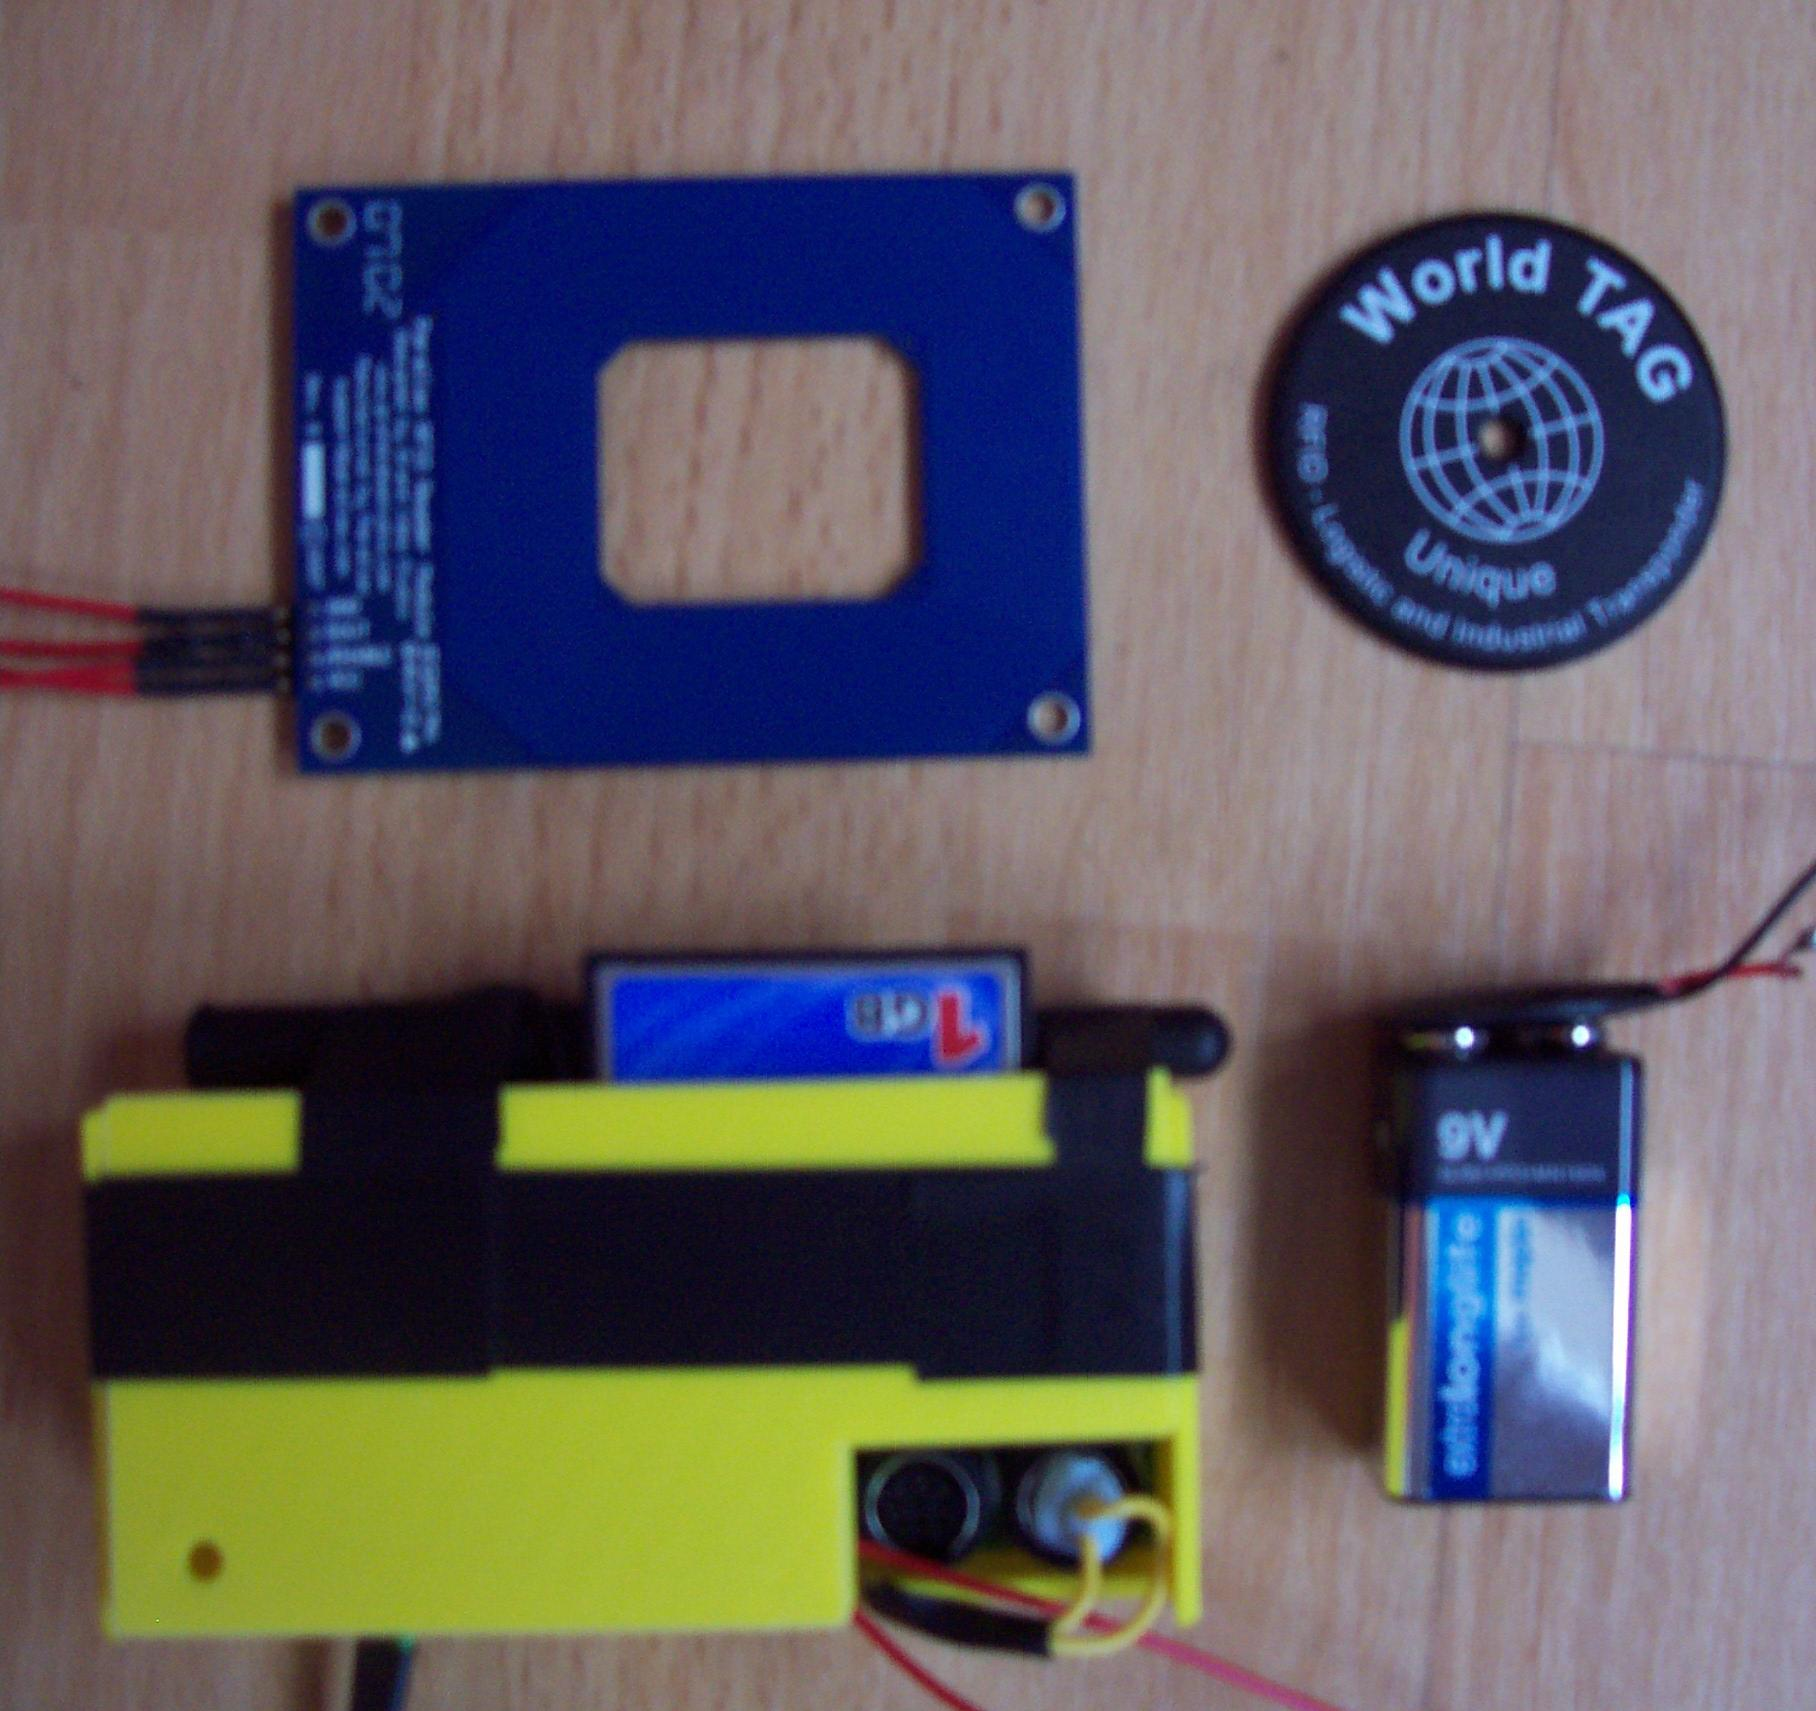
\includegraphics[width=7cm, height=7cm]{mobileShot}
}
\caption{Left) RFID reader to serial circuit, Right) Gumstix connected to RFID reader}
\label{fig:circuit}
\end{figure} 

\begin{figure}[h!]
\centering
\fboxsep 1mm
\framebox{
	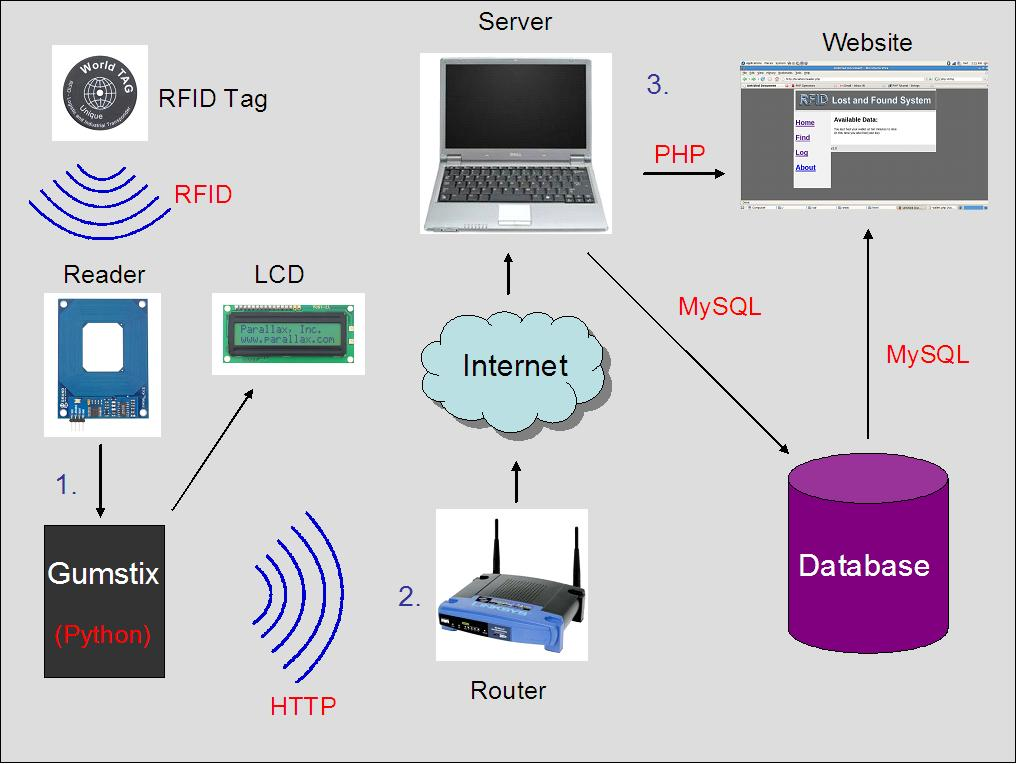
\includegraphics[width=15cm, height=10cm]{architecture}
}
\caption{System Architecture: 1) Gumstix connected to RFID reader and LCD, 2) Router wirelessly receives data from Gumstix, 3) Laptop server hosting database and Lost and Found website}
\label{fig:architecture}
\end{figure} 

Once an RFID tag comes into range of the reader and its ID is read successfully, the ID is taken in by the Gumstix. The Gumstix then transmits this ID wirelessly to a server where it can be stored in a database(step 2 in figure~\ref{fig:architecture}). The function of the server is to host the online lost and found website and a database. The database stores the information which has been wirelessly transmitted by the Gumstix (step 3 in figure~\ref{fig:architecture}). The server runs on a laptop connected to a router. This allows the Gumstix to be configured to connect to the router and use it to transmit data to the server and store it in the database.

Connected to the Gumstix is a 32 character LCD screen. The purpose of this is to enhance the user to system interaction. The LCD connects to one of the Gumstix's serial ports.  The LCD screen is connected to the serial port via a second circuit. This circuit regulates a 5V power supply to power the LCD screen. Figure~\ref{fig:schematic1} shows the schematic for this circuit. The Gumstix transfers data through this circuit which is displayed on the screen as text. Based on objects that have been identified by the RFID reader, the LCD continues to display the last time the user had certain items. Although this information is not as detailed as that presented through the lost and found website, it offers the user assistance in situations where a computer is unavailable. Figure~\ref{fig:architecture} shows the system architecture.

\section{Data Processing}
ReFInDer requires a server used to host the Lost and Found website and database. The server setup used in this project is known as Linux Apache MySQL PHP (LAMP). The LAMP server system consists of a number of open source software technologies which are commonly used together in server applications. It consists of an Apache server~\footnote{Apache website: \url{http://www.apache.org/}}, MySQL~\footnote{MySQL website: \url{www.mysql.com}} for managing databases, and PHP~\footnote{PHP website: \url{http://www.php.net/}} scripting language used for server side data processing in dynamic web pages. These technologies are running on a Linux operating system. The LAMP system was chosen as it encapsulates the required software technologies for the lost and found application. MySQL facilitates the storage and retrieval of tag read data which is transmitted to the server by the mobile component. This data is stored in a MySQL database. The Apache server hosts the webpages which are written using PHP. PHP allows interaction with the MySQL database, such as storing and retrieving data, and processes this information displaying it to the user through the website. See figure~\ref{fig:dataflow} for a data flow diagram.

\begin{figure}[h]
\centering
\fboxsep 1mm
\framebox{
	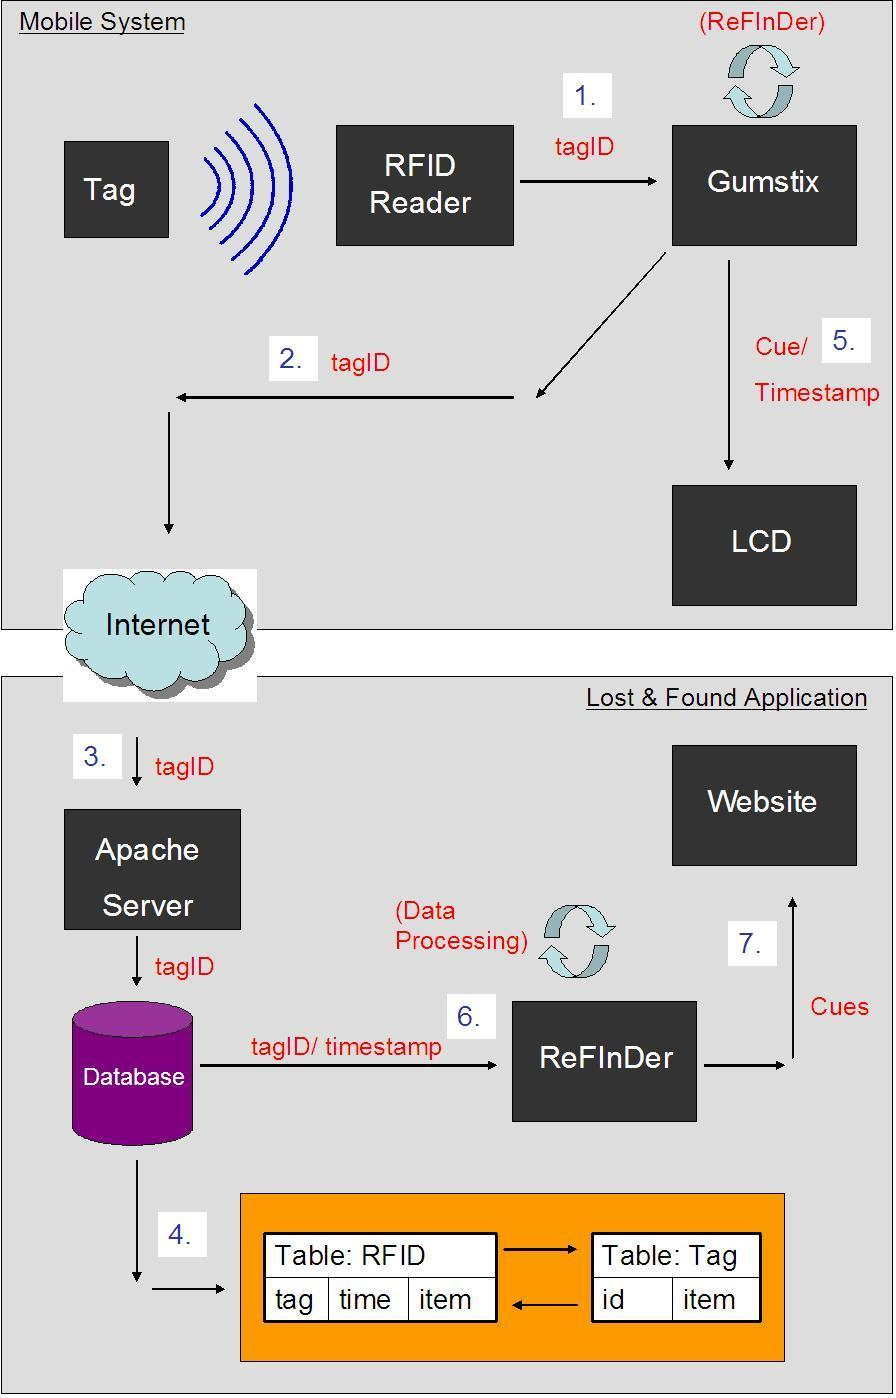
\includegraphics[width=12cm, height=14cm]{dataflow} 
}
\caption{Data Flow Diagram}
\label{fig:dataflow}
\end{figure}

When the Gumstix is powered and boots up, it runs a Python script. The Python script is responsible for transmitting tag IDs to the server which have been read by the RFID reader. It is also responsible for displaying information on the LCD screen. When a tagged object is read by the RFID reader, its ID is passed through the serial port to the Gumstix, (step 1 in figure~\ref{fig:dataflow}). This ID is taken in by the Python script. The Python script can then transmit this ID to a PHP page running on the LAMP server. This PHP page is responsible for storing the tag ID in the database. When a tag is read, its ID is transmitted wirelessly via the router to the PHP page,(step 2 and 3 in figure~\ref{fig:dataflow}). This ID is stored in a database using MySQL queries embedded within the PHP page. Each ID is given a time stamp when it is stored, consisting of the current time and date. When storing a tag ID it is necessary to establish what item the ID corresponds to. Each item that can be identified by the system, such as a phone, has its own unique ID. When storing a new tag ID it is checked against a second database. The second database stores all tag ID's recognised by the system and what item the ID corresponds to. When a tag ID is stored, this information is used to determine which item the ID belongs to and store the corrseponding item name with the tag ID, (step 4 in figure~\ref{fig:dataflow}). For example, the tag ID `04162B761F' is received by the server and PHP page. This ID is checked against the second database which indicates that `04162B761F' corresponds to `phone'. This ID can then be stored with its item name and is given a timestamp, consisting of the current date and time.  

Each time a tag ID is read on the Gumstix, the Python program stores the last occurance of the item. Each time an object is identified its time stamp is updated, so that the system records when you last had that object. Using this information, the Python script sends this data to the LCD screen and displays it in the form of a simple cue, (step 5 in figure~\ref{fig:dataflow}).

\section{User Interfaces}
With RFID data stored, a PHP website can incorporate this as part of the lost and found application. When a user loses an item they simply logon to this website and select the item they are looking for. Using PHP with MySQL the website can retrieve relevant information from the database. This data is presented to the user aiding them in remembering when and where they last had the item, (step 6 and 7 in figure~\ref{fig:dataflow}). One of the goals for this system is to return this information in the form of human readable cues, or in such a way that is as close as possible to human readable language. For example, `You last had your wallet at two o clock.' At this time you were also interacting with your keys�. This is achieved within the PHP pages, formatting and filtering data, and displaying relevant information in the form of the human readable cues. The aim of using human readable cues is to create an application which people can easily relate to. It is the opinion of this author that a person can better relate to natural human language rather than lists of data consisting of dates, times and IDs. The user can read a simple line of text rather than deciphering lists of data in order to obtain useful information. This however may not always be true. The effectiveness of the two data representations, human readable cues and a more technical representation, is discussed in chapter~\ref{evaluations}. Based on the information obtained from these evaluations the lost and found application presents data in both forms. Figure \ref{fig:webshot} shows a screen shot from the web site, which displays an example of the human readable cues.

\begin{figure}[h]
\centering
\fboxsep 2mm
\framebox{
	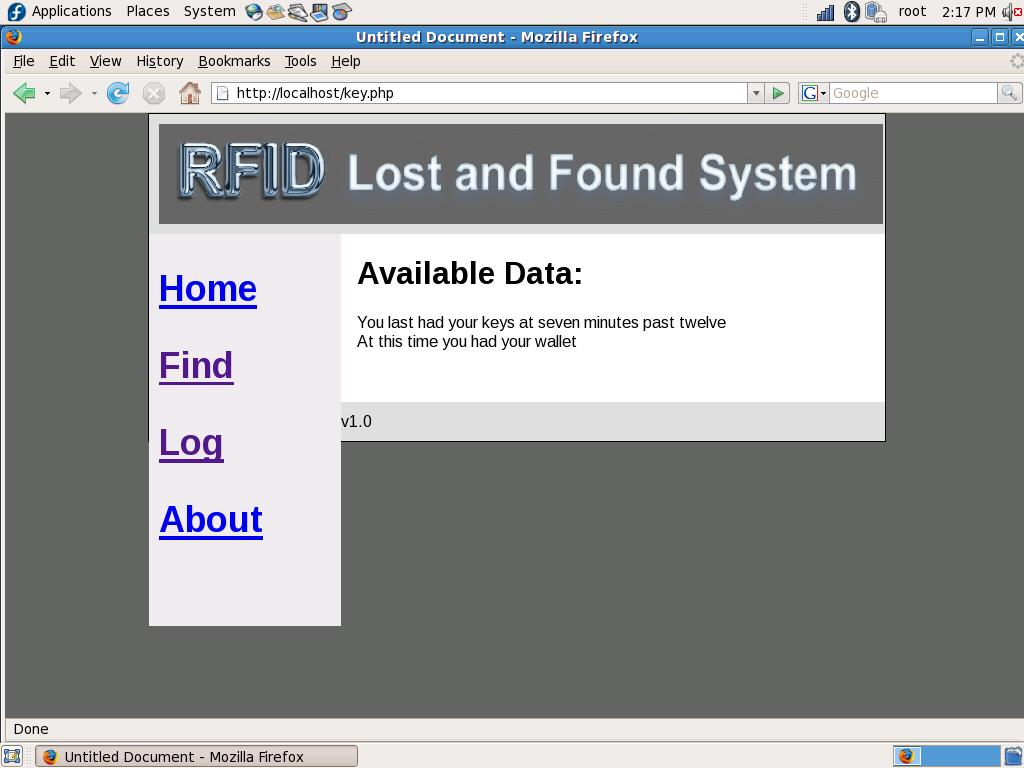
\includegraphics[width=14cm, height=9cm]{websiteShot}
}
\caption{Lost and Found website [Note: will be updated]}
\label{fig:webshot}

\end{figure} 

The second means of presenting useful information to the user is through the LCD screen built into the mobile component. The LCD continues to display the last time you had certain items. Due to the LCD's limited screen space, consisting of 32 characters, the cues are simpler than those found on the lost and found website, for example, `Last had phone @ 17:38, 17/04/2008'. A second limitation with the screen is that users cannot interact with it. They do not have control over the information which is displayed, the system simply cycles through available information. While there are limitations to the LCD screen, the presented information still facilitates user assistance in the situation where a computer is unavailable. 

\section{Bluetooth}
An alternate method of gathering information about a user's activities was explored using Bluetooth. The Gumstix incorporates a built in Bluetooth module which could potentially be used to augment the system's current functionality. The goal of this was to use the Bluetooth module to scan for mobile phone Bluetooth IDs. These IDs could be used to represent people the user has come in contact with. The idea behind gathering this data is to increase the amount of information given to the user through the Lost and Found website. By giving the user more information about their activities, the system could potentially be more effective at helping the user locate an item. In exploring this concept the technology proved ineffective (see appendix \ref{bluetooth} for a discussion of this).

\section{Full System Overview}
The goal of this work is to design and create a Lost and Found application which helps people locate lost items. Two main components are required to achieve this. A mobile component and the Lost and Found application. The mobile component is carried by the user and is responsible for gathering information about a user's interactions with items. To gather this information the mobile component requires a means of retrieving data and wirelessly transmitting it to the Lost and Found Application. Using RFID technology the mobile component can identify when the user has specific items. Items can be identified by placing an RFID tag on them which can be read by the RFID reader. The Gumstix computer facilitates the retrieval of tag IDs from the RFID reader and wirelessly transmitting them to the Lost and Found application running on a server. A Python script running on the Gumstix is responsible for reading in tag IDs from the reader and transmitting them to the server.

The Lost and Found application consists of a website and database hosted on the server. This website is used to view information about lost items. When a tag ID is transmitted by the Gumstix to the server it is stored in a database. When storing a tag ID in the database it is given a timestamp, consisting of the current date and time, and an item name. The item name indicates what item the ID corresponds, such as a wallet. The website retrieves information from this database and displays it to the user in the form of cues, such as `You last had your keys at a quarter past five. At this time you had your phone'. Retrieving information from the database and displaying it in the form of cues is achieved using PHP and MySQL. 
  
\newpage

\chapter{System Testing and Evaluation}
\label{evaluations}

\section{Introduction}
The ideal evaluation for the ReFInDer system would be a longitudinal study as done by Logan et al.\cite{beth}, which involved a house rigged with different sensing equipment. This study resulted in a lot of data and took weeks for full evaluation. For ReFInDer this would involve a user trial in which a person uses the system for a long period of time and the system's performance is evaluated over this period. Due to the fact that ReFInDer is currently a proof of concept prototype, which can only be self powered for short periods of time from 9v batteries. For any effective long term evaluation the system must be kept plugged into the mains, which is completely impractical for a full user trial. Also due to the fact that there is currently only one prototype and a lack of resources to effectively carry out such a trial, the next best evaluation process has been taken. Individual testing has been undertaken in each of the ReFInDer system's key components. 

\section{RFID Prototype}
\label{evaluationsprototype}
Early system testing began with a working prototype implementing the RFID component. This consisted of the RFID reader connected to the Gumstix, setup of the LAMP server, and implementation of a simple lost and found website. This prototype was designed to evaluate a number of key components of the system. The circuit built for relaying tag IDs to the Gumstix serial port included an LED, which was used to indicate when tags were being read successfully. To ensure tag read data was being transferred successfully to the server a simple test page was setup, which retrieved the contents of the database and displayed it on screen. The evaluation consisted of placing tags near the RFID reader and moving it slowly closer along a ruler. This was tested using the front, back, and sides of the reader, with 20 readings taken for each. The goal of this was to determine if items could be identified with their ID successfully transmitted to the database. The ruler was used to evaluate the range limitations of the reader, indicating at what distances tags could be accurately read. 

Three tag types were used in this evaluation. The first tag was a rectanglur shape measuring 54mm x 85.5mm and is 0.8mm thick, which are identical dimensions to most credit cards. The RFID reader's documentation indicates that this tag should have an average readable range of approximately 6.3cm. The documentation indicated that this measurement was based on positioning the face of the tag parallel to the front or back face of the reader. The second tag was a circular shape measuring 50mm in diamater and 2.1mm thick. The suggested readable range for this tag was 6.8cm. The last tag was also circular measuring 25mm in diameter and 1mm thick, roughly the size of a one euro coin. There was no suggested readable range for this tag type. Figure \ref{fig:tags!} shows the three tag types used in the evaluation. Figure \ref{fig:rfidproto} shows a photo of the evaluation and the php test page.

\begin{figure}[h]
\centering
\fboxsep 1mm
\framebox{
	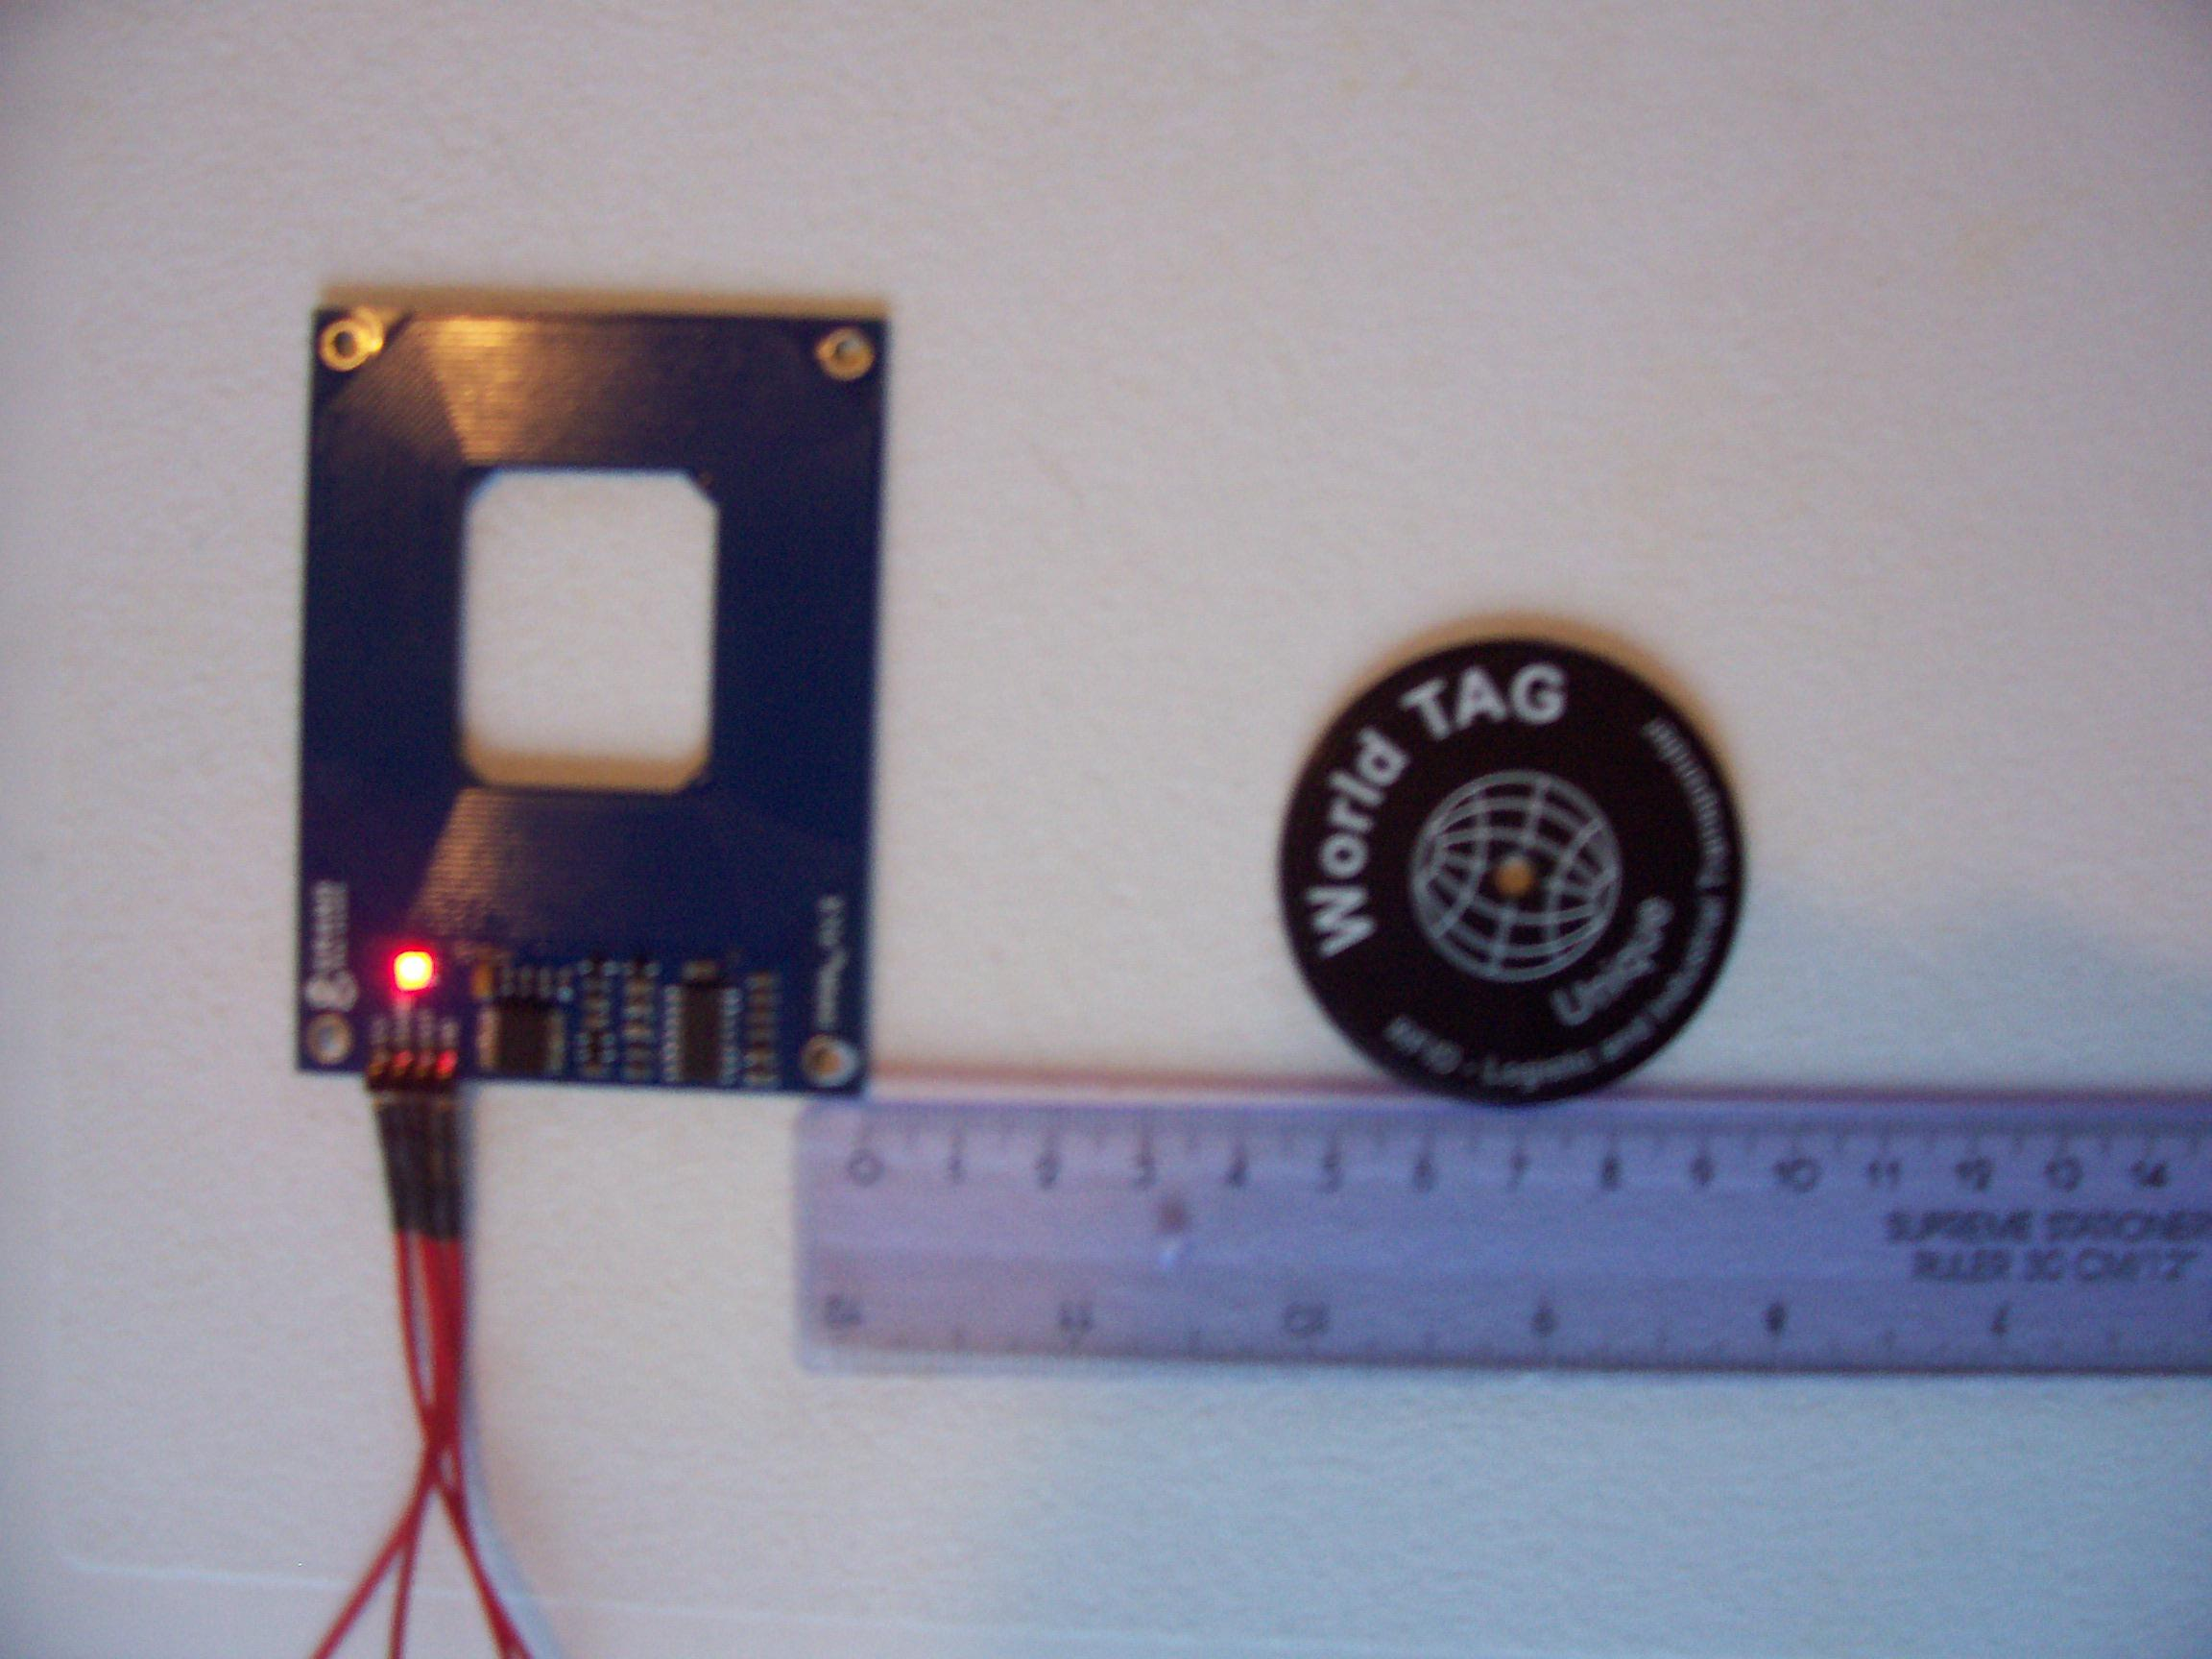
\includegraphics[width=7.5cm, height=5.5cm]{protoshot} 
	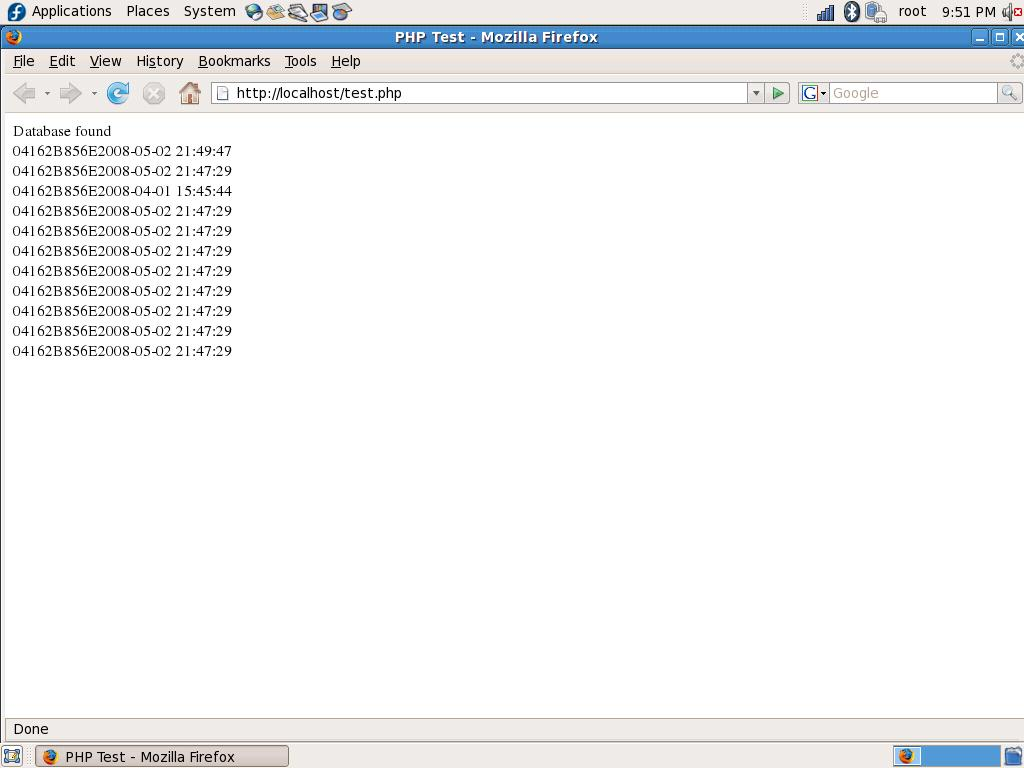
\includegraphics[width=7.5cm, height=5.5cm]{protoscreen}
}
\caption{RFID Prototype Evaluation: Left) RFID reader and 50mm circular tag, Right) Screenshot of testing webpage}
\label{fig:rfidproto}
\end{figure} 

\begin{figure}[h]
\centering
\fboxsep 1mm
\framebox{
	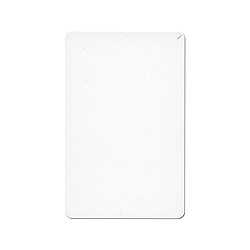
\includegraphics[width=5cm, height=5cm]{tag1} 
	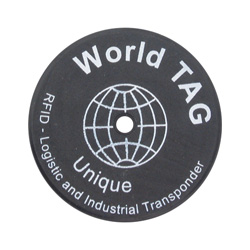
\includegraphics[width=5cm, height=5cm]{tag2}
	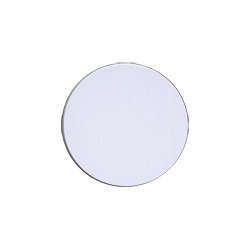
\includegraphics[width=5cm, height=5cm]{tag3}
}
\caption{RFID Tags: Left) Rectangular Tag, Center) Circular Tag (50mm), Left) Circular Tag (25mm)\cite{parallax}}
\label{fig:tags!}
\end{figure} 

\subsection{Results}
The following table shows the results from the evaluation of the RFID reader's range. It shows the mean readable range of each tag type for the front, back, and sides of the RFID reader. For each of the front, back, and sides, the standard deviation (SD) of the obtained results are given.
\begin{center}
\begin{tabular}{ | l || c | c || c | c || c | c || }
\hline			
Tag Type & Front & SD & Back & SD & Sides & SD \\ \hline
Rectangular Tag & 6.5cm & 0.5 & 6.3cm & 0.4cm & 3.3cm & 0.4cm \\
Circular Tag: 50mm & 8.9cm & 3.2cm & 8.2cm & 1.9cm & 3.9cm & 2.2cm \\
Circular Tag: 25mm & 3.3cm & 0.3cm & 2.8cm & 0.4cm & 1.2cm & 0.4cm \\
\hline  
\end{tabular}
\end{center}

The results of this evaluation higlighted the limitations of the RFID reader's range. However it was found that once a tag is within this range it is accurately identified. Viewing the test page, which displayed the contents of the database, indicated that once an ID is read, it is always transmitted and stored correctly in the database. This was confirmed using the testing webpage and the LED light incorporated into the circuit which connects the RFID reader to the Gumstix. The LED flashes to indicate that the circuit is receiving data. The testing webpage displays the contents of the database. Viewing this webpage indicated that the tag reads had been successfully transmitted and stored in the database. This indicates that the hardware setup and data processing techniques are sound, however the readers range needed to be considered. 

\section{System Form Factor}
\label{evaluationsform}
The goal of the system's form factor is to create a system which is small, compact and easily carried by the user. The second factor in its design was the address the limitations of the readers range. A small pouch design can be placed within a pocket or bag along with other items. Due to the relatively small space of pockets and bags, items are in close proximity to each other at all times. The aim of this test was to determine if this can overcome the readers limitations. 

Although the system is very compact and portable it is necessary to highlight that it is a \textit{proof of concept}. If such a system was designed and built commercially it would be considerably smaller and lighter. For example the Gumstix computer is much more powerful than is necessary for the data processing involved in the system. The circuits involved for connecting components could be constructed using printed circuit boards which would also be considerably smaller in size. The weight of the form factor is mainly due to the two 9V batteries it contains. Again a commercially built system could feature a smaller and lower weight battery. 

This evaluation involved placing the pouch inside the pocket of a bag and a jacket. Tagged objects were placed in the pocket with the pouch in different combinations and positions in order to determine if they could be identified successfully. Tagged objects consisted of a wallet, phone and a set of keys. The RFID reader is positioned at the back of the pouch, as seen in figure \ref{fig:pouch}. For this reason it was necessary to evaluate its effectiveness at reading tags from both the front and back of the pouch. In the evaluation the pouch was tested 30 times for each side.   

\subsection{Results}
The results of the form factor evaluation were promising but also highlighted a potential weakness in its design. When placed in a pocket, ReFInDer successfully identified tagged items 27 out of 30 tests as long as the reader was facing toward them. If the pouch was positioned the wrong way around it was found that the system was less effective, with 13 of 30 tests identifying a tagged item. These results indicate that the form factor is very effective when used in a specific way, however if the pouch was placed in a pocket incorrectly it considerably less accurate.

To evaluate the form factor it was placed in both a bag and a jacket pocket. The bag provided ample space to fit the ReFInDer system along with a number of items however when placed in a jacket pocket the extra space was limited. It was not possible to comfortably fit more than one or two small tagged item in the pocket with the pouch.
  
\section{Human Readable Cues}
To evaluate the human readable cues a survey was created to gather feedback on which technique people consider more effective, the human readable cues or raw data consisting of date and time stamps. This was issued to 13 third year computer science students who had no direct association with the project. To eliminate the possibility that computer science students may have a certain bias towards more complicated and detailed data, based on their experience with working with this type of data, the survey was also issued to 10 non computer science students. See appendix \ref{survey} for the survey. 

\subsection{Results}
The results from the survey showed much similarity in peoples' opinions of each data representation. Strong conclusions could therefore be drawn from the results and were used to influence how data is presented on the lost and found website. In the survey basic cues consisted of lists of time stamps and the corresponding item that you had at this time, e.g., `2008-04-01 16:51:31: key'. See figure \ref{fig:cueex} for an example of the two data representations. The survey indicated a number of advantages and disadvantages with this data representation. 12 out of 13 computer science students considered there to be disadvantages with this representation. Responses included: \textit{`This could be seen as too much effort to decipher', `It's not very easy to understand', `Slightly difficult to read since it's just a list of numbers', `Could take a while to interpret and draw conclusions', `It's a lot of data. Some users might feel this is overwhelming', `Hard to read for someone not used to it', `From a user point of view, I would rather see a simple line of text than read lines of date/time/item', `It's long and not very personal'}. Of the 12 participants who considered there to be disadvantages of this format, 10 out of 12 considered this format difficult to read or time consuming to interpret the results. Results were similar from the 10 non computer science students. 10 out of 10 participants considered there to be disadvantages with this data type. Responses included, \textit{`Potentially complicated', `Didnt really understand it at first', `Might be hard to follow if there is lots of things', `Its a little hard to read'.} 

\begin{figure}[h]
\centering
\fboxsep 1mm
\framebox{
	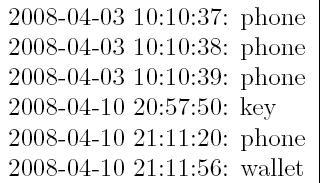
\includegraphics[width=6cm, height=4cm]{cuea} 
	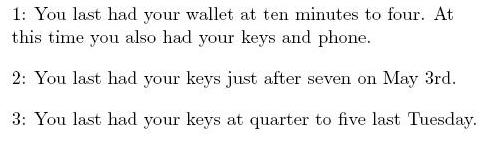
\includegraphics[width=9cm, height=4cm]{cueb}
}
\caption{Cue Formats: Left) A: Basic cues, Right) B: Human readable cues }
\label{fig:cueex}
\end{figure}

Advantages were offered in 12 out of 13 computer science students. Responses included, \textit{`The sequence of events is easy to see', `Could be used to map patterns to the usual places where you keep something', `Gives all the information', `Precise', `It shows multiple interactions with one item', `You can see more information'.} Of these 12 participants 6 considered this representation more precise or informative, 5 of the 12 participants felt more detailed information about a user's activities could be derived. 8 out of 10 non computer science students considered there to be advantages of this data representation. Responses included, \textit{`More detailed', `Theres a lot more information', `Concise', `Not too hard after you look at it a few times'.}

With regards to the more human readable cues, participants were again asked the advantages and disadvantages of this format. An example of this format is, `You last had your wallet at ten minutes to four. At this time you also had your keys and phone'. Of the 13 computer science students 11 considered there to be disadvantages, this included, \textit{`Not as precise', `Doesn't show surrounding events', `Not very precise, can seem vague', `Not as much times shown', `Lacks the amount of information provided in A'.} The advantages of this format were found to be very similar. Responses included, \textit{`Much more straightforward, easier to obtain required info', `Much easier to read than A', `B has a personal touch, it would be a lot easier to read', `Very basic, straightforward, easy to understand'.} Of the 10 non computer science students 8 considered there to be disadvantages. \textit{`Not as much detail', `Seems like you dont get all the facts', `Lack of past history', `Cant trace back'.} 

12 out of 13 computer science students felt there was advantages of this format. \textit{`Simple, basic, shown in one line', `Straightforward, easy to understand', `Easy to read and understand', `Intuitive and easy to understand'.} 9 out of 10 non computer science students also thought there were advantages, with every response stating that it was either easier to read or easier to understand.

Participants were also asked to compare each format to the other, and if they considered one more advantageous to the other. In 7 out of 13 cases of the computer science participants considered there to be advantages to both formats, with no strong advantage of one format over the other. Out of 13 responses, 3 people considered basic cues more advantageous and 3 preferred the human readable cues. Some insightful responses included, \textit{`Overall, I think B is more advantageous to a random person, also it is not as overwhelming', `B would be better to introduce to individuals who are not technofiles and are wary of using new technology', `B would be easier to understand until you're used to the layout of A', `Presenting both representations would be helpful. If B is not enough information, A could be looked at'.} Results from the non computer science students were very similar. 2 out of 10 participants preferred the basic cues, \textit{`I prefer A because I can just glance at it and see exactly where I my things', `A gives more information than B so I prefer that one'.} 3 out of 10 participants indicated that they preferred the human readable cues, and 5 out of 10 considered there to be advantages to both formats.

The results for both computer science students and non computer science students were very similar. This eliminates the possibility of bias towards either data representation. Overall participants considered the basic cues to be more difficult to read and time consuming to interpret. They are however more precise and offer more detailed information. The more human readable cues were considered easy to read but not as precise and detailed. Initially this author considered the more human readable cues to be more suitable and effective in this type of system. The results, however suggest that there are no strong advantages of this. Each representation of the data offered conflicting advantages and disadvantages over the other. For example basic cues are more precise and the human readable cues are less precise. Some interesting comments suggested that the human readable cues would also be more suitable to people who are not used to technology. The results also suggested that if a person was comfortable with interpreting the detailed information in the basic cues, they could derive more information, such as more effectively tracking their movements. With each format offering its own advantages it was chosen to incorporate both into the lost and found website. As there can be different types of people, those comfortable with using technology and those who are not, the application can offer benefits to a wider audience of users. 

The last survey question was intended to gather any comments or suggestions participants may have. Eight of the overall 23 participants offered suggestions. Responses from this question offered some valid and useful ways that could potentially augment the ReFInDer system's functionality. These are discussed further as future work in section \ref{future2}.     

\newpage

\chapter{Conclusions and Future Work}
\label{future}

\section{Conclusions}
The primary goal of this project was to design a memory aid system using RFID technology and to determine its effectiveness in this task. An important component of the system was the ability to identify objects. The initial system prototype was a basic version of the system, which was designed to test the effectiveness of RFID technology for identifying items. The RFID reader was found to be accurate at identifying tagged objects which suggests that it is a useful and effective technology for implementing such a system. While the effectiveness of reading tags was found to be very accurate the reader did have a limited range. The range was found to be between 2.8cm and 8.9cm, depending on the type of tag being used. This influenced the system's form factor and how the system was used. 

The evaluation of the system's form factor indicated that it was effective when used in a specific way. The back side of the pouch which contains the RFID reader was very accurate at identifying items, however if the front side of the pouch is facing towards tagged items the system performance is lower. This suggests that the approach taken in designing the form factor is sound, however modifications are required to overcome potential shortcomings, and improve overall system accuracy. This evaluation also found that the form factor was not practical to use in a jacket packet. This would indicate that the form factor is too large to be used in this way, and its usability is dependant on the size of the pocket. While it is important for such a system to be compact, the tested implementation is a \textit{proof of concept} prototype and is considerably larger and heavier than would be required in a commercially designed version. For such a system it is important that it is unobtrusive and something which can be used naturally. The user should be almost unaware they are using it. The current size and weight of the prototype is unacceptable in this case. For a commercially designed version of this system, the size and weight would be very important. Due to the fact that the Gumstix is significantly larger and more powerful than is required, combined with the fact that the system circuits could be replaced with printed circuits, a significantly smaller and lightweight commercial implementation is very plausible.

The results of the cue evaluation survey highlighted some important findings with regards to the human readable cues. It was found that the human readable cues were easy to read and the user can get useful information very quickly. However it was also found that they lacked a certain level of detail. The basic cues consisted of time stamps and corresponding items presented in a list. Survey participants considered this format harder to read, however it is still considered much more precise and could potentially be used to derive more information about their activities. Based upon the findings that there are benefits of representing information in different ways it is concluded that it is of benefit to the user that the lost and found application presents information in both formats. This offers benefits for different types of users. 

The overall findings of this work indicate that RFID is an effective and useful technology in this system. This was indicated by the RFID prototype evaluation which showed a high level of accuracy. This supports the findings of Schmidt and Gellerson in their research of the applicability of RFID in wearable computing \cite{schmidt}. While RFID technology is shown to be accurate it was found to be limited in its range. The system's form factor was designed to compensate for this, where the mobile component consisted of a pouch which is placed inside a pocket with tagged items. The results indicated that this was a successful approach, however the pouch needs to be used in a specific way to facilitate accurate tag reading. This is not ideal and indicates that modifications are required to increase the form factors overall usability. Solutions to this are discussed in section \ref{future2}. The goal of the Lost and Found website is to present the user with data recorded by the system through the form of human readable cues. Evaluations of the cues suggest that the human readable cue format is not necessarily the most effective approach. While it was found that there are many advantages to this format for the user, it lacks a certain level of detail. Designing the Lost and Found application offering both the human readable cues and more detailed data, serves to offer more benefits to the user.  

\section{Future Work}
\label{future2}
The built in LCD screen of the ReFInDer's mobile component is a means of improving user and system interaction, offering an alternate means of giving information to the user. The information displayed by the screen is simple due to the screens limited space. Future improvements to this includes more detailed information being displayed to the user. This could perhaps be achieved using a larger screen or by a means of scrolling text across the current screen. Currently users do not have any control over what information is displayed to them through the built in display. Future enhancements to the ReFInDer system could include incorporating control buttons into the mobile component. These buttons could perhaps be used to select specific information, such as information about a specific lost item.

This work explored an alternative means of gathering information about a user's activities using Bluetooth. By representing people based upon their mobile phone Bluetooth ID the system could keep track of people the user came into contact with. The motivation for this was to increase the amount of information recorded by the system thus increasing the amount of useful information given to the user. By giving a user more information about their activities, the system could potentially be more effective at aiding a person's memory. Although difficulties arose in its implementation, this author considers this a viable solution for future improvements to the ReFInDer system. It could be successfully implemented using a stable Gumstix software revision with correctly functioning wireless and Bluetooth capabilities. This revision would also need to satisfy the Gumstix's limited memory constraints. 

A longitudinal study would be the ideal method of evaluating ReFInDer. This would involve a full user trial of the system over a period of weeks to months. Due to a lack of available resources and other factors, undertaking such an evaluation was not feasible. Future evaluations would need to include such a user trial to properly determine ReFInDer's applicability and performance in everyday situations. To effectively implement this study a solution is required with regards to battery life and powering the mobile component. Currently the mobile component can not be powered for long periods of time from 9V batteries and connecting it to the mains would be impractical for the evaluation. A possible solution to this would involve replacing the 9v batteries with higher capacity rechargeable batteries.

Evaluations indicated that the form factor is effective but modifications are necessary to overcome a potential shortcoming. Item identification is very effective from the back side of the pouch where the RFID reader is located, but is very limited from the front side of the pouch. A possible solution to this would involve incorporating a second RFID reader positioned at the front of the pouch. This would overcome the necessity to have the pouch positioned or used in a specific way, however this may shorten battery life. Again higher capacity batteries may be a solution to this.   

In the cue evaluations survey, participants were asked if they had any further comments and suggestions. There are some notable results from this question offering some valid potential improvements for ReFInDer. \textit{`[the first set of cues] could be used to map patterns to the usual places where you keep something'.} In this comment the first set of cues are made up of lists of time stamps and their corresponding item, e.g., `2008-04-11 04:50:03: phone'. This comment suggests using the recorded times and comparing them to where you would normally keep an item at that time. This idea has merit and would perhaps be useful for items such as keys that are kept in a specific location when you are at home, for example. However it is this authors opinion that people do not often keep items in specific locations, especially when not at home. It is also perhaps not as likely to lose an item when at home. An alternate solution would be to compare the recorded time stamps with where you are at certain times. For example, if you work between 09:00 and 17:00 during the day and the system records that you last had your wallet at 15:43, the system could suggest that you may have left your wallet in work. One participant suggested, \textit{`Colour code each item to make [the first set of cues] easier to read at a glance'.} This is a potential solution to make the detailed basic cues easier to read and interpret. From an implementation point of view this would not appear difficult to implement. 

Another reply to this question was, \textit{`A voice interaction with [the second set of cues] would be cool, especially to, perhaps, older people'}. In this comment the second set of cues are the more human readable cues, such as `You last had your wallet at ten minutes to four. At this time you also had your keys and phone'. This suggestion could be a potentially useful way of improving the system's user interface. Older people may be somewhat uncomfortable with using technology however the Lost and Found application is currently very simple to use, with easy website navigation where users simply click on what item they are looking for. For this reason voice recognition could be considered unnecessary functionality. Perhaps a future survey evaluation would provide more insight into this. 
\newpage

\appendix
\chapter{Cue Evaluation Survey}
\label{survey}

\section{Introduction}
The purpose of this survey was to evaluate the human readable cues. The survey presents two formats for representing the information gathered by ReFInDer. In the survey, participants are asked if they consider there to be any advantages or disadvantages to each of the two data representations. They are also asked to compare the two, specifically if they consider one data type to be more advantageous over the other. The final question asks participants if they have any further comments or suggestions.


\subsection{Survey}
\begin{center}
"Using RFID to remember": Human readable cues evaluation
\end{center}

The purpose of this project is to create a memory aid, which helps people find lost items. It does this by gathering information about a person's interactions with items. It records when people were interacting with such items and stores this information. This information is used by a website. When a user loses something they log into this website where they are presented with this information. This information is displayed in the form of readable cues. An example of a readable cue would be: "You last had your watch at 16:45". 

Below are two ways of representing the cues, A and B.
  
A: Basic cues

\begin{tabular}{ | l | l | }
\hline			
2008-04-01 15:45:43: phone & 2008-04-01 16:51:31: key \\
2008-04-01 15:45:44: phone & 2008-04-01 16:51:32: key \\
2008-04-01 15:45:48: phone & 2008-04-01 16:51:33: key \\
2008-04-01 16:06:37: phone & 2008-04-01 16:55:27: phone \\
2008-04-01 16:06:38: phone & 2008-04-01 16:55:31: phone \\
2008-04-01 16:18:15: key & 2008-04-01 16:55:32: phone \\
2008-04-01 16:18:16: key & 2008-04-01 16:55:32: phone \\
2008-04-01 16:18:16: key & 2008-04-02 12:34:14: key \\
2008-04-01 16:18:17: key & 2008-04-03 10:10:31: key \\
2008-04-01 16:18:19: key & 2008-04-03 10:10:32: key \\
2008-04-01 16:18:20: key & 2008-04-03 10:10:32: key \\
2008-04-01 16:18:20: key & 2008-04-03 10:10:37: phone \\
2008-04-01 16:34:24: wallet & 2008-04-03 10:10:37: phone \\
2008-04-01 16:34:25: wallet & 2008-04-03 10:10:38: phone \\
2008-04-01 16:34:25: wallet & 2008-04-03 10:10:39: phone \\
2008-04-01 16:34:26: wallet & 2008-04-10 20:57:50: key \\
2008-04-01 16:34:27: wallet & 2008-04-10 21:11:20: phone \\
2008-04-01 16:34:28: wallet & 2008-04-10 21:11:56: wallet \\
2008-04-01 16:34:29: wallet & 2008-04-12 03:50:12: wallet \\
\hline  
\end{tabular}

B: Human readable cues

	
1: You last had your phone at ten past ten, April 3rd. 

2: You last had your keys at two minutes to nine pm.

3: You last had your wallet at eleven minutes past nine. \\At this time you had your wallet.



Q1: What would you consider are the advantages and disadvantages of the way data is represented in A?

Q2: What would you consider are the advantages and disadvantages of the way data is represented in B?

Q3: From the two data representations what would you consider the relative benefits of A vs. B? For example are there advantages of using one method over the other? 

Q4: Do you have any further comments or suggestions?

\chapter{Bluetooth}
\label{bluetooth}
After the main components of ReFInDer had been implemented the Gumstix was looked at in more detail. It contains an integrated Bluetooth module which could be used to explore an alternative means of gathering information about a user's activities. It was proposed that this could potentially be used to identify people the user has come into contact with based upon their Bluetooth phone ID. From an implementation point of view this would involve modifying the Python script responsible for transmitting RFID tag IDs to also scan for Bluetooth devices and transmit their unique ID using the same technique. To achieve this Python requires a Bluetooth API which allow it to utilise the Gumstix's Bluetooth capabilities. The Gumstix does not include this functionality as default which meant it was necessary to add new software to the Gumstix.   

To add new software to a Gumstix a special program is required called Buildroot~\footnote{Buildroot information can be found here: \url{http://buildroot.uclibc.org/}}. Buildroot is used to generate root filesystems for Linux systems and is not solely Gumstix specific. Buildroot allows users to create a filesystem to run on the Gumstix. Before building the filesystem users select packages or software that you want to run on the Gumstix, such as programming languages like Python. Once desired packages have been selected with Buildroot it compiles and creates a filesystem for the Gumstix which contains all the chosen software and functionality. This filesystem can then be flashed or copied to the Gumstix.

To facilitate the Bluetooth functionality a package named PyBluez was required~\footnote{PyBluez information can be found here: \url{http://org.csail.mit.edu/pybluez/}}. The Buildroot process was very time consuming, taking approximately three hours to build a revision and flash it to the Gumstix over a serial cable. Difficulties arose once the filesystem had been flashed to the Gumstix. There are many revisions or versions of Buildroot, at the time of this writing there are currently 1602 revisions, most of which are not stable and contain bugs. This means certain functionality will not work in all revisions. For example one revision may have Bluetooth support but its wireless capabilities will not work correctly. It was essential for the ReFInDer system to have wireless capabilities for transmitting data. Experimenting with different revisions of Buildroot failed to result in a stable version that offered both wireless and Bluetooth support. Due to the sheer number of revisions and lack of available information on stable versions, coupled with the lengthy build process for each tested Buildroot revision, experimenting with random selections was not a viable solution. Attempts were made to take a revision of Buildroot with wireless functionality and replace its Bluetooth packages with those from a revision that had working Bluetooth support, however this was unsuccessful. The issue of unstable Buildroot revisions is a well known issue, with much discussion in related forums and blogs~\footnote{Gumstix Forum Discussions: \url{http://www.nabble.com/forum/Search.jtp?forum=22543&local=y&query=stable+buildroot}}~\footnote{Gumstix Mailing List Archive: \url{http://article.gmane.org/gmane.linux.distributions.gumstix.general/30503/match=stable+buildroot}}~\footnote{Hindenstix blog: \url{http://hindenstix.blogspot.com/2008/04/09-frustrated-flashing.html}}, however at the time of writing no viable solution to this problem has emerged.

A second difficulty with Buildroot was the size of the generated filesystem and the Gumstix memory constraints. The Gumstix has two memory types, RAM and flash memory. The flash memory is 16mb, and stores the Linux filesystem. The filesystem generated by Buildroot must be less than this. Experimenting with newer versions of the Buildroot generated filesystems which were far too large to use. This appeared to be due to an increase in Buildroots core components. 

Although augmenting the ReFInDer system's data gathering techniques and functionality using Bluetooth is a valid approach the technology proved somewhat ineffective in this case.

%%%% ADD YOUR BIBLIOGRAPHY HERE
\newpage
\begin{thebibliography}{99}
\bibitem{intel}
	  Roy Want,
	  \emph{An Introduction to RFID Technology}.
	  IEEE Pervasive Computing 5, 1 (Jan. 2006), 25.
	  
	\bibitem{intel2}
	  Matthai Philipose, Kenneth P. Fishkin, Mike Perkowitz, Donald J. Patterson, Dieter Fox, Henry Kautz, and Dirk Hahnel,
	  \emph{Inferring Activities from Interactions with Objects}.
	  IEEE Pervasive Computing 3, 4 (Oct. 2004), 50-57.  
	  
	 \bibitem{intel3}
	  Kenneth P. Fishkin, Matthai Philipose, and Adam Rea, 2005.
	  \emph{Hands-On RFID: Wireless Wearables for Detecting Use of Objects}.
	  Proceedings of the Ninth IEEE international Symposium on Wearable Computers (October 18 - 21, 2005). ISWC. IEEE Computer Society, Washington, DC, 38-43.
	  
	  \bibitem{wong}
	  Kirk H. Wong, Patrick. C. Hui, and Allan C. Chan, 2006. 
	  \emph{Cryptography and authentication on RFID passive tags for apparel products.}.
	  Comput. Ind. 57, 4 (May. 2006), 342-349.
	   
	  \bibitem{ece}
	  Suppakrit Chatchayanuson, Charles Christopher Oneyama, Nachiket Shelgikar, Saravana Sivasankaran 
	  \emph{Kitchen Tracker}.
	  Electrical and Computer Engineering, Carnagie Mellon University, 2007.
	  
	  \bibitem{ubi}
	  Tatsuyuki Kawamura, Tomohiro Fukuhara, Hideaki Takeda, Yasuyuki Kono, and Masatsugu Kidode 
	  \emph{Ubiquitous Memories: a memory externalization system using physical objects}.
	  Personal Ubiquitous Comput. 11, 4 (Apr. 2007), 287-298. 
	  
	  \bibitem{smart}
	  Alex S. Taylor, Richard Harper, Laurel Swan, Shahram Izadi, Abigail Sellen, and Mark Perry
	  \emph{Homes that make us Smart}.
	  Personal Ubiquitous Comput. 11, 5 (Jun. 2007), 383-393.  
	  
	  \bibitem{cait}
	  Caitlin Lustig, Lorcan Coyle
	  \emph{Reminding Short-Term Memory Sufferers to Complete Routine Tasks}.
	  Technical Report UCD-CSI-2007-10, 2007, UCD Dublin
	  
	  \bibitem{cait2}
	  Caitlin Lustig, Hristo Novatchkov, Lucy E. Dunne, Mike McHugh, and Lorcan Coyle (2007).
	  \emph{Using Colocation to Support Human Memory. Workshop "Supporting Human Memory with Interactive Systems"}.
	  HCI Conference, September 4th, 2007, Lancaster, UK. Pages 41-44
	  
	  \bibitem{schmidt}
	  Albrecht Schmidt, Christian Merz, and Hans-W. Gellerson
	  \emph{Enabling implicit human computer interaction- a wearable rfid-tag reader}.
	  Proc. 4th Int'l Symp. Wearable Computers (ISWC2000), pp. 193-194
	  
	  \bibitem{weiser}
	  Mark Weiser
	  \emph{The Computer for the 21st Century}.
	  SIGMOBILE Mob. Comput. Commun. Rev. 3, 3 (Jul. 1999), 3-11.
	  
	  \bibitem{beth}
	  Beth Logan, Jennifer Healey, Matthai Philipose, Emmanuel Munguia Tapia, Stephen S. Intille
	  \emph{A Long-Term Evaluation of Sensing Modalities for Activity Recognition}.
	  Ubicomp 2007: 483-500 
	  
	  \bibitem{jamie}
	  Jamie A. Ward, Paul Lukowicz, Gerhard Tr�ster, Thad Starner
	  \emph{Activity Recognition of Assembly Tasks Using Body-Worn Microphones and Accelerometers}.
	  IEEE Trans. Pattern Anal. Mach. Intell. 28(10): 1553-1567 (2006)
	  
	  \bibitem{parallax}
	  \emph{Parallax Home}.
	  http://www.parallax.com/ (April 16, 2008)
	  
	  \bibitem{dey}
	  Anind K. Dey, Peter Ljungstrand, and Albrecht Schmidt
	  \emph{Distributed and disappearing user interfaces in ubiquitous computing.}.
	  CHI '01 Extended Abstracts on Human Factors in Computing Systems (Seattle, Washington, March 31 - April 05, 2001). CHI '01. ACM, New York, NY, 487-488.
	  	  
\end{thebibliography}
\label{endpage}


\end{document}

\end{article}
